\section{Controle Modular Local}

\begin{frame}{Metodologia Utilizada}

    \Large \textbf{Controle Modular Local:}
    \normalsize

    \vspace{2mm}

    
Dividir para conquistar! Assumindo que a modelagem das plantas já tenha sido obtida, os passos necessários para aplicação do Controle Modular Local podem ser sintetizados como segue
    

    \begin{itemize}
        \item \textbf{1º:} Definição de plantas assíncronas.
        \item \textbf{2º:} Composição paralela das subplantas assíncronas.
        \item \textbf{3º:} Aplicação do comportamento especificado para cada subsistema.
    \end{itemize}

\end{frame}

\begin{frame}{Metodologia Utilizada}

    \begin{itemize}
        \item \textbf{Definição do plano de ação para subplantas e restrições respectivas:}
    \end{itemize}

    \begin{figure}[htbp]
        \centering
        \resizebox{0.53\textwidth}{!}{


\tikzset{every picture/.style={line width=0.75pt}} %set default line width to 0.75pt        

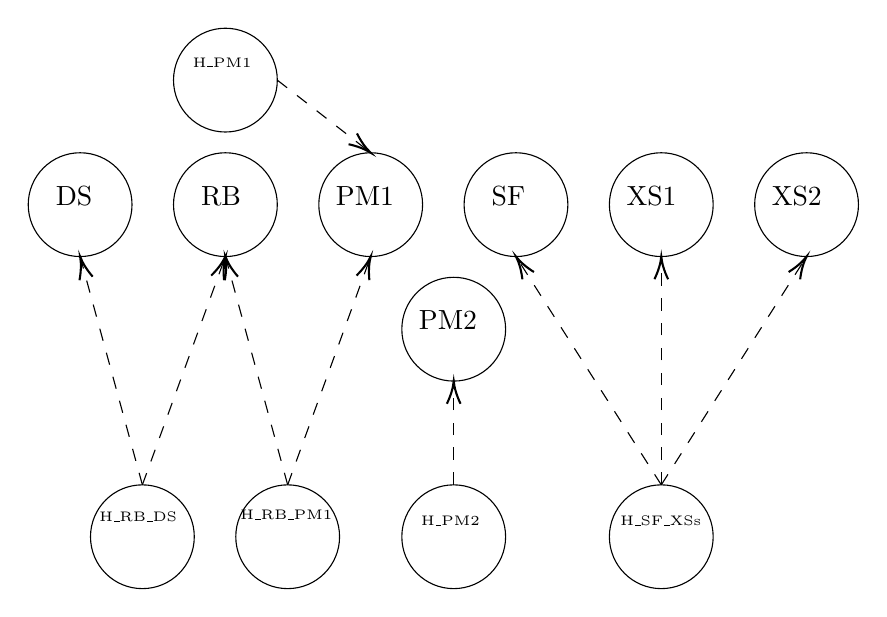
\begin{tikzpicture}[x=0.75pt,y=0.75pt,yscale=-1,xscale=1]
%uncomment if require: \path (0,300); %set diagram left start at 0, and has height of 300

%Shape: Circle [id:dp22427385377578068] 
\draw   (340,105) .. controls (340,91.19) and (351.19,80) .. (365,80) .. controls (378.81,80) and (390,91.19) .. (390,105) .. controls (390,118.81) and (378.81,130) .. (365,130) .. controls (351.19,130) and (340,118.81) .. (340,105) -- cycle ;
%Shape: Circle [id:dp8451597487753835] 
\draw   (200,105) .. controls (200,91.19) and (211.19,80) .. (225,80) .. controls (238.81,80) and (250,91.19) .. (250,105) .. controls (250,118.81) and (238.81,130) .. (225,130) .. controls (211.19,130) and (200,118.81) .. (200,105) -- cycle ;
%Shape: Circle [id:dp9851423637089443] 
\draw   (270,105) .. controls (270,91.19) and (281.19,80) .. (295,80) .. controls (308.81,80) and (320,91.19) .. (320,105) .. controls (320,118.81) and (308.81,130) .. (295,130) .. controls (281.19,130) and (270,118.81) .. (270,105) -- cycle ;
%Shape: Circle [id:dp2739284496312233] 
\draw   (310,165) .. controls (310,151.19) and (321.19,140) .. (335,140) .. controls (348.81,140) and (360,151.19) .. (360,165) .. controls (360,178.81) and (348.81,190) .. (335,190) .. controls (321.19,190) and (310,178.81) .. (310,165) -- cycle ;
%Shape: Circle [id:dp01596519258680895] 
\draw   (410,105) .. controls (410,91.19) and (421.19,80) .. (435,80) .. controls (448.81,80) and (460,91.19) .. (460,105) .. controls (460,118.81) and (448.81,130) .. (435,130) .. controls (421.19,130) and (410,118.81) .. (410,105) -- cycle ;
%Shape: Circle [id:dp0658111958460239] 
\draw   (480,105) .. controls (480,91.19) and (491.19,80) .. (505,80) .. controls (518.81,80) and (530,91.19) .. (530,105) .. controls (530,118.81) and (518.81,130) .. (505,130) .. controls (491.19,130) and (480,118.81) .. (480,105) -- cycle ;
%Shape: Circle [id:dp7699962639330244] 
\draw   (130,105) .. controls (130,91.19) and (141.19,80) .. (155,80) .. controls (168.81,80) and (180,91.19) .. (180,105) .. controls (180,118.81) and (168.81,130) .. (155,130) .. controls (141.19,130) and (130,118.81) .. (130,105) -- cycle ;
%Shape: Circle [id:dp23709629916496056] 
\draw   (230,265) .. controls (230,251.19) and (241.19,240) .. (255,240) .. controls (268.81,240) and (280,251.19) .. (280,265) .. controls (280,278.81) and (268.81,290) .. (255,290) .. controls (241.19,290) and (230,278.81) .. (230,265) -- cycle ;
%Straight Lines [id:da8393258077310075] 
\draw  [dash pattern={on 4.5pt off 4.5pt}]  (185,240) -- (155.53,131.93) ;
\draw [shift={(155,130)}, rotate = 74.74] [color={rgb, 255:red, 0; green, 0; blue, 0 }  ][line width=0.75]    (10.93,-3.29) .. controls (6.95,-1.4) and (3.31,-0.3) .. (0,0) .. controls (3.31,0.3) and (6.95,1.4) .. (10.93,3.29)   ;
%Straight Lines [id:da772763632121459] 
\draw  [dash pattern={on 4.5pt off 4.5pt}]  (185,240) -- (224.32,131.88) ;
\draw [shift={(225,130)}, rotate = 109.98] [color={rgb, 255:red, 0; green, 0; blue, 0 }  ][line width=0.75]    (10.93,-3.29) .. controls (6.95,-1.4) and (3.31,-0.3) .. (0,0) .. controls (3.31,0.3) and (6.95,1.4) .. (10.93,3.29)   ;
%Straight Lines [id:da49281506852447454] 
\draw  [dash pattern={on 4.5pt off 4.5pt}]  (255,240) -- (225.53,131.93) ;
\draw [shift={(225,130)}, rotate = 74.74] [color={rgb, 255:red, 0; green, 0; blue, 0 }  ][line width=0.75]    (10.93,-3.29) .. controls (6.95,-1.4) and (3.31,-0.3) .. (0,0) .. controls (3.31,0.3) and (6.95,1.4) .. (10.93,3.29)   ;
%Straight Lines [id:da1517351405395171] 
\draw  [dash pattern={on 4.5pt off 4.5pt}]  (435,240) -- (366.07,131.69) ;
\draw [shift={(365,130)}, rotate = 57.53] [color={rgb, 255:red, 0; green, 0; blue, 0 }  ][line width=0.75]    (10.93,-3.29) .. controls (6.95,-1.4) and (3.31,-0.3) .. (0,0) .. controls (3.31,0.3) and (6.95,1.4) .. (10.93,3.29)   ;
%Straight Lines [id:da9900732811154345] 
\draw  [dash pattern={on 4.5pt off 4.5pt}]  (255,240) -- (294.32,131.88) ;
\draw [shift={(295,130)}, rotate = 109.98] [color={rgb, 255:red, 0; green, 0; blue, 0 }  ][line width=0.75]    (10.93,-3.29) .. controls (6.95,-1.4) and (3.31,-0.3) .. (0,0) .. controls (3.31,0.3) and (6.95,1.4) .. (10.93,3.29)   ;
%Straight Lines [id:da3226489467563065] 
\draw  [dash pattern={on 4.5pt off 4.5pt}]  (435,240) -- (435,132) ;
\draw [shift={(435,130)}, rotate = 90] [color={rgb, 255:red, 0; green, 0; blue, 0 }  ][line width=0.75]    (10.93,-3.29) .. controls (6.95,-1.4) and (3.31,-0.3) .. (0,0) .. controls (3.31,0.3) and (6.95,1.4) .. (10.93,3.29)   ;
%Straight Lines [id:da812653243494788] 
\draw  [dash pattern={on 4.5pt off 4.5pt}]  (435,240) -- (503.93,131.69) ;
\draw [shift={(505,130)}, rotate = 122.47] [color={rgb, 255:red, 0; green, 0; blue, 0 }  ][line width=0.75]    (10.93,-3.29) .. controls (6.95,-1.4) and (3.31,-0.3) .. (0,0) .. controls (3.31,0.3) and (6.95,1.4) .. (10.93,3.29)   ;
%Shape: Circle [id:dp5138680940136209] 
\draw   (160,265) .. controls (160,251.19) and (171.19,240) .. (185,240) .. controls (198.81,240) and (210,251.19) .. (210,265) .. controls (210,278.81) and (198.81,290) .. (185,290) .. controls (171.19,290) and (160,278.81) .. (160,265) -- cycle ;
%Shape: Circle [id:dp2284217374383941] 
\draw   (410,265) .. controls (410,251.19) and (421.19,240) .. (435,240) .. controls (448.81,240) and (460,251.19) .. (460,265) .. controls (460,278.81) and (448.81,290) .. (435,290) .. controls (421.19,290) and (410,278.81) .. (410,265) -- cycle ;
%Shape: Circle [id:dp21687728838899445] 
\draw   (200,45) .. controls (200,31.19) and (211.19,20) .. (225,20) .. controls (238.81,20) and (250,31.19) .. (250,45) .. controls (250,58.81) and (238.81,70) .. (225,70) .. controls (211.19,70) and (200,58.81) .. (200,45) -- cycle ;
%Shape: Circle [id:dp18160666688593685] 
\draw   (310,265) .. controls (310,251.19) and (321.19,240) .. (335,240) .. controls (348.81,240) and (360,251.19) .. (360,265) .. controls (360,278.81) and (348.81,290) .. (335,290) .. controls (321.19,290) and (310,278.81) .. (310,265) -- cycle ;
%Straight Lines [id:da052747497553948364] 
\draw  [dash pattern={on 4.5pt off 4.5pt}]  (335,240) -- (335,192) ;
\draw [shift={(335,190)}, rotate = 90] [color={rgb, 255:red, 0; green, 0; blue, 0 }  ][line width=0.75]    (10.93,-3.29) .. controls (6.95,-1.4) and (3.31,-0.3) .. (0,0) .. controls (3.31,0.3) and (6.95,1.4) .. (10.93,3.29)   ;
%Straight Lines [id:da08290066885446357] 
\draw  [dash pattern={on 4.5pt off 4.5pt}]  (250,45) -- (293.42,78.77) ;
\draw [shift={(295,80)}, rotate = 217.87] [color={rgb, 255:red, 0; green, 0; blue, 0 }  ][line width=0.75]    (10.93,-3.29) .. controls (6.95,-1.4) and (3.31,-0.3) .. (0,0) .. controls (3.31,0.3) and (6.95,1.4) .. (10.93,3.29)   ;

% Text Node
\draw (352,95) node [anchor=north west][inner sep=0.75pt]   [align=left] {SF};
% Text Node
\draw (212,95) node [anchor=north west][inner sep=0.75pt]   [align=left] {RB};
% Text Node
\draw (277,95) node [anchor=north west][inner sep=0.75pt]   [align=left] {PM1};
% Text Node
\draw (317,155) node [anchor=north west][inner sep=0.75pt]   [align=left] {PM2};
% Text Node
\draw (417,95) node [anchor=north west][inner sep=0.75pt]   [align=left] {XS1};
% Text Node
\draw (487,95) node [anchor=north west][inner sep=0.75pt]   [align=left] {XS2};
% Text Node
\draw (142,95) node [anchor=north west][inner sep=0.75pt]   [align=left] {DS};
% Text Node
\draw (231,251) node [anchor=north west][inner sep=0.75pt]   [align=left] {{\tiny H\_RB\_PM1}};
% Text Node
\draw (163,252) node [anchor=north west][inner sep=0.75pt]   [align=left] {{\tiny H\_RB\_DS}};
% Text Node
\draw (208,33) node [anchor=north west][inner sep=0.75pt]   [align=left] {{\tiny H\_PM1}};
% Text Node
\draw (318,254) node [anchor=north west][inner sep=0.75pt]   [align=left] {{\tiny H\_PM2}};
% Text Node
\draw (414,254) node [anchor=north west][inner sep=0.75pt]   [align=left] {{\tiny H\_SF\_XSs}};


\end{tikzpicture}}
        \caption{Subplantas e suas respectivas restrições.}
        \label{fig:SFXSs} 
    \end{figure}


\end{frame}

\begin{frame}{Definição de plantas assíncronas.}

    \begin{itemize}
        \item \textbf{Individualização de cada componente} 
    \end{itemize}

    

    \begin{figure}[htbp]
        \centering
        \resizebox{0.4\textwidth}{!}{


\tikzset{every picture/.style={line width=0.75pt}} %set default line width to 0.75pt        

\begin{tikzpicture}[x=0.75pt,y=0.75pt,yscale=-1,xscale=1]
%uncomment if require: \path (0,2709); %set diagram left start at 0, and has height of 2709

%Image [id:dp5010384262434795] 
\draw (835,240) node  {\includegraphics[width=315pt,height=300pt]{tikz/modelo/modelo.png}};

% Text Node
\draw (670,85) node  [font=\large] [align=left] {\begin{minipage}[lt]{41.14pt}\setlength\topsep{0pt}
\begin{center}
SF
\end{center}

\end{minipage}};
% Text Node
\draw (750,85) node  [font=\large] [align=left] {\begin{minipage}[lt]{41.14pt}\setlength\topsep{0pt}
\begin{center}
RB
\end{center}

\end{minipage}};
% Text Node
\draw (900,130) node  [font=\large] [align=left] {\begin{minipage}[lt]{41.14pt}\setlength\topsep{0pt}
\begin{center}
PM1
\end{center}

\end{minipage}};
% Text Node
\draw (680,250) node  [font=\large] [align=left] {\begin{minipage}[lt]{41.14pt}\setlength\topsep{0pt}
\begin{center}
DS
\end{center}

\end{minipage}};
% Text Node
\draw (680,410) node  [font=\large] [align=left] {\begin{minipage}[lt]{41.14pt}\setlength\topsep{0pt}
\begin{center}
XS1
\end{center}

\end{minipage}};
% Text Node
\draw (995,270) node  [font=\large] [align=left] {\begin{minipage}[lt]{41.14pt}\setlength\topsep{0pt}
\begin{center}
XS2
\end{center}

\end{minipage}};
% Text Node
\draw (835,320) node  [font=\large] [align=left] {\begin{minipage}[lt]{41.14pt}\setlength\topsep{0pt}
\begin{center}
PM2
\end{center}

\end{minipage}};


\end{tikzpicture}}
        \caption{Planta para a máquina de \textit{milkshake}.}
        \label{fig:sistema}
    \end{figure}
    

\end{frame}


\begin{frame}{Composição paralela das subplantas assíncronas.}

    \begin{itemize}
        \item \textbf{Modelagem individual de cada componente;} 
    \end{itemize}

    Plantas com restrições individuais

    \begin{itemize}
        \item \textit{Processing Machine 1}
        \item \textit{Processing Machine 2}
    \end{itemize}

    Ambas restrições são independentes, e ligeiramente diferentes, e comandam o \textbf{ciclo de funcionamento} das \textit{Processing Machines}, que trabalham de forma autônoma ao resto do sistema executam suas respectivas ações - de enchimento com \textit{milkshake} e cobertura - uma vez que o sensor acuse a chegada do copo.


\end{frame}

\begin{frame}{\textit{Processing Machine} (PM1).}

    Restricão para a subplanta composta apenas da \textit{Processing Machine 1}.

    \begin{figure}[htbp]
        \centering
        \resizebox{0.7\textwidth}{!}{


\tikzset{every picture/.style={line width=0.75pt}} %set default line width to 0.75pt        

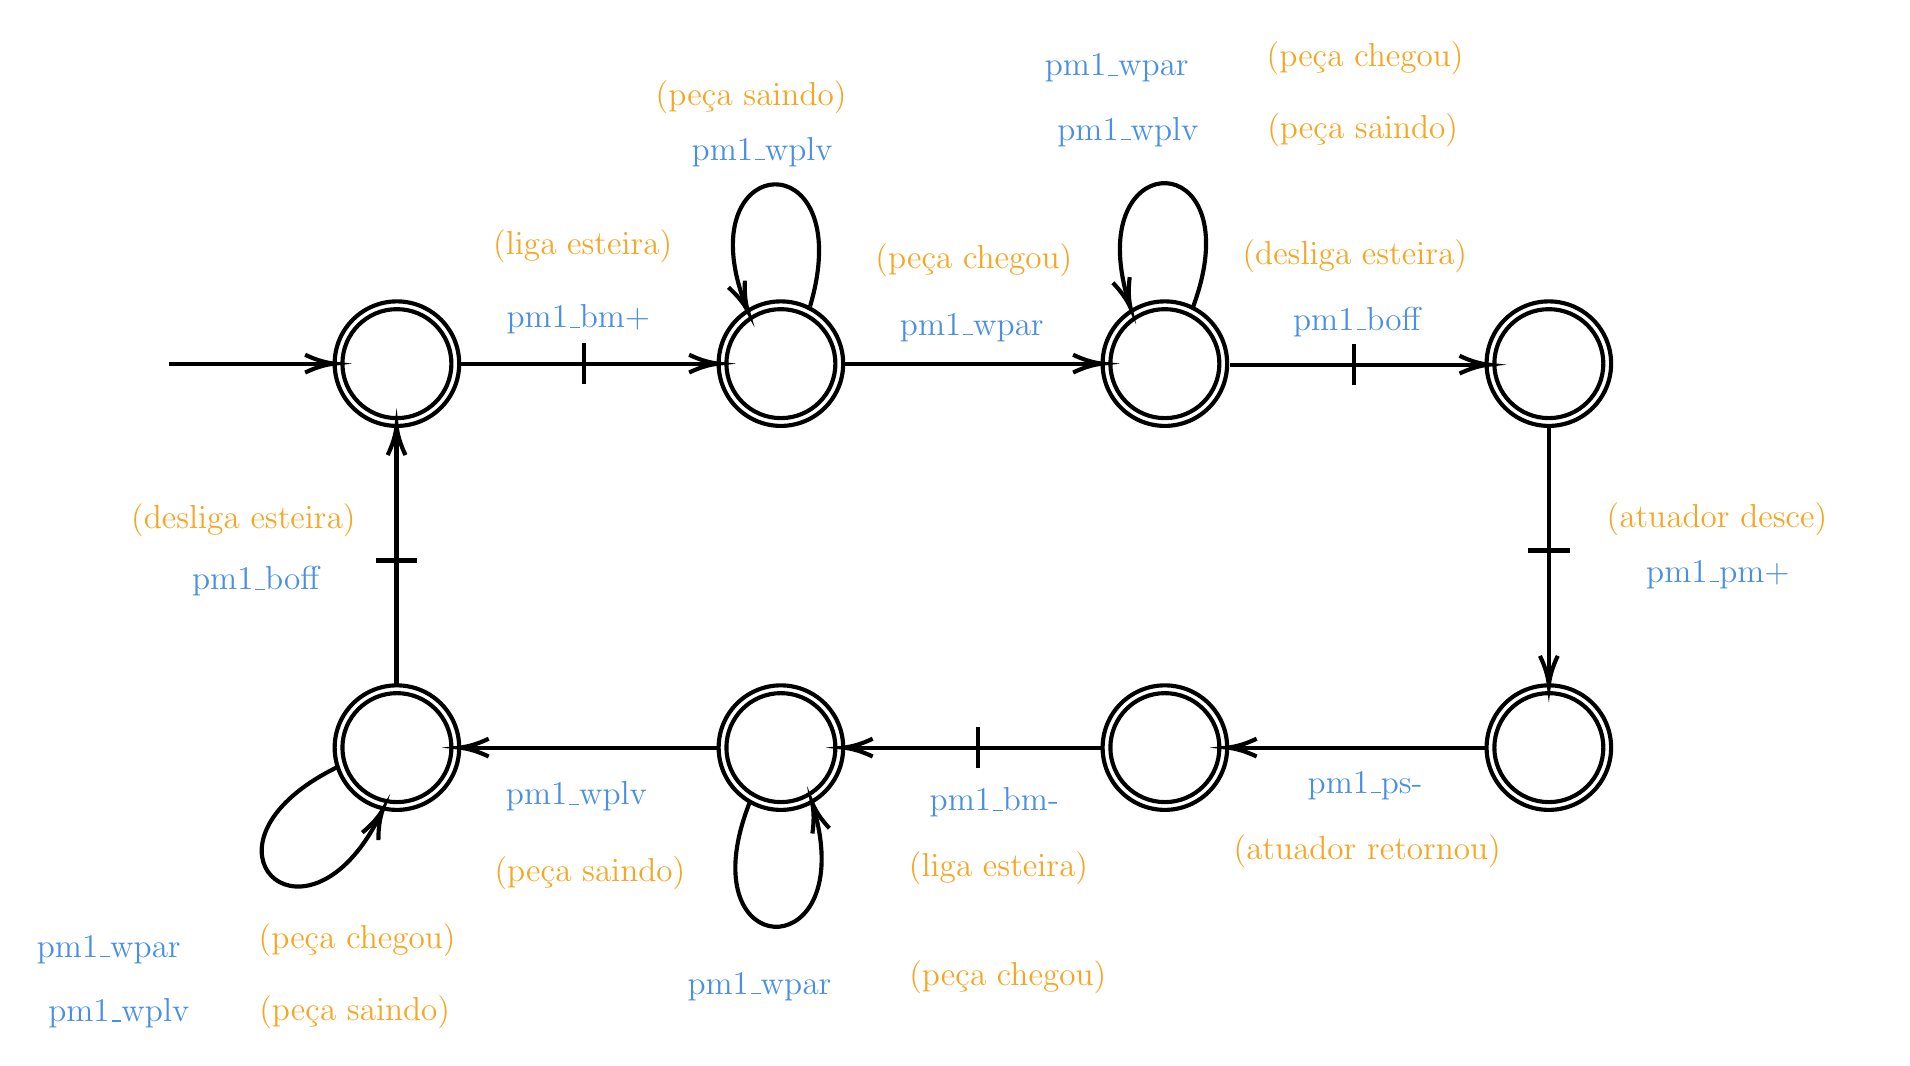
\begin{tikzpicture}[x=0.75pt,y=0.75pt,yscale=-1,xscale=1]
%uncomment if require: \path (0,3420); %set diagram left start at 0, and has height of 3420

%Shape: Circle [id:dp5021231821953818] 
\draw  [line width=1.5]  (1371.5,2916.5) .. controls (1371.5,2899.93) and (1384.93,2886.5) .. (1401.5,2886.5) .. controls (1418.07,2886.5) and (1431.5,2899.93) .. (1431.5,2916.5) .. controls (1431.5,2933.07) and (1418.07,2946.5) .. (1401.5,2946.5) .. controls (1384.93,2946.5) and (1371.5,2933.07) .. (1371.5,2916.5) -- cycle ;
%Shape: Circle [id:dp5289461805073701] 
\draw  [line width=1.5]  (1375.25,2916.5) .. controls (1375.25,2902) and (1387,2890.25) .. (1401.5,2890.25) .. controls (1416,2890.25) and (1427.75,2902) .. (1427.75,2916.5) .. controls (1427.75,2931) and (1416,2942.75) .. (1401.5,2942.75) .. controls (1387,2942.75) and (1375.25,2931) .. (1375.25,2916.5) -- cycle ;
%Straight Lines [id:da4788090574749646] 
\draw [line width=1.5]    (1291.5,2916.5) -- (1368.5,2916.5) ;
\draw [shift={(1371.5,2916.5)}, rotate = 180] [color={rgb, 255:red, 0; green, 0; blue, 0 }  ][line width=1.5]    (14.21,-4.28) .. controls (9.04,-1.82) and (4.3,-0.39) .. (0,0) .. controls (4.3,0.39) and (9.04,1.82) .. (14.21,4.28)   ;
%Straight Lines [id:da8018832314051378] 
\draw [line width=1.5]    (1431.5,2916.5) -- (1454.5,2916.5) -- (1553.5,2916.5) ;
\draw [shift={(1556.5,2916.5)}, rotate = 180] [color={rgb, 255:red, 0; green, 0; blue, 0 }  ][line width=1.5]    (14.21,-4.28) .. controls (9.04,-1.82) and (4.3,-0.39) .. (0,0) .. controls (4.3,0.39) and (9.04,1.82) .. (14.21,4.28)   ;
%Straight Lines [id:da0076803473792970145] 
\draw [line width=1.5]    (1491.5,2906.5) -- (1491.5,2926.5) ;

%Shape: Circle [id:dp22625731925102777] 
\draw  [line width=1.5]  (1556.5,2916.5) .. controls (1556.5,2899.93) and (1569.93,2886.5) .. (1586.5,2886.5) .. controls (1603.07,2886.5) and (1616.5,2899.93) .. (1616.5,2916.5) .. controls (1616.5,2933.07) and (1603.07,2946.5) .. (1586.5,2946.5) .. controls (1569.93,2946.5) and (1556.5,2933.07) .. (1556.5,2916.5) -- cycle ;
%Straight Lines [id:da9270365039391677] 
\draw [line width=1.5]    (1616.5,2916.5) -- (1738.5,2916.5) ;
\draw [shift={(1741.5,2916.5)}, rotate = 180] [color={rgb, 255:red, 0; green, 0; blue, 0 }  ][line width=1.5]    (14.21,-4.28) .. controls (9.04,-1.82) and (4.3,-0.39) .. (0,0) .. controls (4.3,0.39) and (9.04,1.82) .. (14.21,4.28)   ;
%Shape: Circle [id:dp8790830623806889] 
\draw  [line width=1.5]  (1741.5,2916.5) .. controls (1741.5,2899.93) and (1754.93,2886.5) .. (1771.5,2886.5) .. controls (1788.07,2886.5) and (1801.5,2899.93) .. (1801.5,2916.5) .. controls (1801.5,2933.07) and (1788.07,2946.5) .. (1771.5,2946.5) .. controls (1754.93,2946.5) and (1741.5,2933.07) .. (1741.5,2916.5) -- cycle ;
%Shape: Circle [id:dp05996581087867403] 
\draw  [line width=1.5]  (1926.5,2916.5) .. controls (1926.5,2899.93) and (1939.93,2886.5) .. (1956.5,2886.5) .. controls (1973.07,2886.5) and (1986.5,2899.93) .. (1986.5,2916.5) .. controls (1986.5,2933.07) and (1973.07,2946.5) .. (1956.5,2946.5) .. controls (1939.93,2946.5) and (1926.5,2933.07) .. (1926.5,2916.5) -- cycle ;
%Straight Lines [id:da8561532153311397] 
\draw [line width=1.5]    (1956.5,2946.5) -- (1956.5,2969.5) -- (1956.5,3068.5) ;
\draw [shift={(1956.5,3071.5)}, rotate = 270] [color={rgb, 255:red, 0; green, 0; blue, 0 }  ][line width=1.5]    (14.21,-4.28) .. controls (9.04,-1.82) and (4.3,-0.39) .. (0,0) .. controls (4.3,0.39) and (9.04,1.82) .. (14.21,4.28)   ;
%Straight Lines [id:da5406403779740838] 
\draw [line width=1.5]    (1966.5,3006.5) -- (1946.5,3006.5) ;

%Shape: Circle [id:dp1389806805521474] 
\draw  [line width=1.5]  (1926.5,3101.5) .. controls (1926.5,3084.93) and (1939.93,3071.5) .. (1956.5,3071.5) .. controls (1973.07,3071.5) and (1986.5,3084.93) .. (1986.5,3101.5) .. controls (1986.5,3118.07) and (1973.07,3131.5) .. (1956.5,3131.5) .. controls (1939.93,3131.5) and (1926.5,3118.07) .. (1926.5,3101.5) -- cycle ;
%Straight Lines [id:da3566574988633957] 
\draw [line width=1.5]    (1804.5,3101.5) -- (1926.5,3101.5) ;
\draw [shift={(1801.5,3101.5)}, rotate = 0] [color={rgb, 255:red, 0; green, 0; blue, 0 }  ][line width=1.5]    (14.21,-4.28) .. controls (9.04,-1.82) and (4.3,-0.39) .. (0,0) .. controls (4.3,0.39) and (9.04,1.82) .. (14.21,4.28)   ;
%Shape: Circle [id:dp5939143750931828] 
\draw  [line width=1.5]  (1741.5,3101.5) .. controls (1741.5,3084.93) and (1754.93,3071.5) .. (1771.5,3071.5) .. controls (1788.07,3071.5) and (1801.5,3084.93) .. (1801.5,3101.5) .. controls (1801.5,3118.07) and (1788.07,3131.5) .. (1771.5,3131.5) .. controls (1754.93,3131.5) and (1741.5,3118.07) .. (1741.5,3101.5) -- cycle ;
%Shape: Circle [id:dp9635042203289415] 
\draw  [line width=1.5]  (1556.5,3101.5) .. controls (1556.5,3084.93) and (1569.93,3071.5) .. (1586.5,3071.5) .. controls (1603.07,3071.5) and (1616.5,3084.93) .. (1616.5,3101.5) .. controls (1616.5,3118.07) and (1603.07,3131.5) .. (1586.5,3131.5) .. controls (1569.93,3131.5) and (1556.5,3118.07) .. (1556.5,3101.5) -- cycle ;
%Shape: Circle [id:dp022192289610075466] 
\draw  [line width=1.5]  (1371.5,3101.5) .. controls (1371.5,3084.93) and (1384.93,3071.5) .. (1401.5,3071.5) .. controls (1418.07,3071.5) and (1431.5,3084.93) .. (1431.5,3101.5) .. controls (1431.5,3118.07) and (1418.07,3131.5) .. (1401.5,3131.5) .. controls (1384.93,3131.5) and (1371.5,3118.07) .. (1371.5,3101.5) -- cycle ;
%Straight Lines [id:da8665047753384527] 
\draw [line width=1.5]    (1741.5,3101.5) -- (1718.5,3101.5) -- (1619.5,3101.5) ;
\draw [shift={(1616.5,3101.5)}, rotate = 360] [color={rgb, 255:red, 0; green, 0; blue, 0 }  ][line width=1.5]    (14.21,-4.28) .. controls (9.04,-1.82) and (4.3,-0.39) .. (0,0) .. controls (4.3,0.39) and (9.04,1.82) .. (14.21,4.28)   ;
%Straight Lines [id:da33313592666384406] 
\draw [line width=1.5]    (1681.5,3111.5) -- (1681.5,3091.5) ;

%Shape: Circle [id:dp323983994895517] 
\draw  [line width=1.5]  (1560.25,2916.5) .. controls (1560.25,2902) and (1572,2890.25) .. (1586.5,2890.25) .. controls (1601,2890.25) and (1612.75,2902) .. (1612.75,2916.5) .. controls (1612.75,2931) and (1601,2942.75) .. (1586.5,2942.75) .. controls (1572,2942.75) and (1560.25,2931) .. (1560.25,2916.5) -- cycle ;
%Shape: Circle [id:dp061991462662711605] 
\draw  [line width=1.5]  (1745.25,2916.5) .. controls (1745.25,2902) and (1757,2890.25) .. (1771.5,2890.25) .. controls (1786,2890.25) and (1797.75,2902) .. (1797.75,2916.5) .. controls (1797.75,2931) and (1786,2942.75) .. (1771.5,2942.75) .. controls (1757,2942.75) and (1745.25,2931) .. (1745.25,2916.5) -- cycle ;
%Shape: Circle [id:dp8712457883247433] 
\draw  [line width=1.5]  (1930.25,2916.5) .. controls (1930.25,2902) and (1942,2890.25) .. (1956.5,2890.25) .. controls (1971,2890.25) and (1982.75,2902) .. (1982.75,2916.5) .. controls (1982.75,2931) and (1971,2942.75) .. (1956.5,2942.75) .. controls (1942,2942.75) and (1930.25,2931) .. (1930.25,2916.5) -- cycle ;
%Shape: Circle [id:dp4032269267721291] 
\draw  [line width=1.5]  (1930.25,3101.5) .. controls (1930.25,3087) and (1942,3075.25) .. (1956.5,3075.25) .. controls (1971,3075.25) and (1982.75,3087) .. (1982.75,3101.5) .. controls (1982.75,3116) and (1971,3127.75) .. (1956.5,3127.75) .. controls (1942,3127.75) and (1930.25,3116) .. (1930.25,3101.5) -- cycle ;
%Shape: Circle [id:dp7865107563162004] 
\draw  [line width=1.5]  (1745.25,3101.5) .. controls (1745.25,3087) and (1757,3075.25) .. (1771.5,3075.25) .. controls (1786,3075.25) and (1797.75,3087) .. (1797.75,3101.5) .. controls (1797.75,3116) and (1786,3127.75) .. (1771.5,3127.75) .. controls (1757,3127.75) and (1745.25,3116) .. (1745.25,3101.5) -- cycle ;
%Shape: Circle [id:dp6415554207822463] 
\draw  [line width=1.5]  (1560.25,3101.5) .. controls (1560.25,3087) and (1572,3075.25) .. (1586.5,3075.25) .. controls (1601,3075.25) and (1612.75,3087) .. (1612.75,3101.5) .. controls (1612.75,3116) and (1601,3127.75) .. (1586.5,3127.75) .. controls (1572,3127.75) and (1560.25,3116) .. (1560.25,3101.5) -- cycle ;
%Shape: Circle [id:dp25769850815519857] 
\draw  [line width=1.5]  (1375.25,3101.5) .. controls (1375.25,3087) and (1387,3075.25) .. (1401.5,3075.25) .. controls (1416,3075.25) and (1427.75,3087) .. (1427.75,3101.5) .. controls (1427.75,3116) and (1416,3127.75) .. (1401.5,3127.75) .. controls (1387,3127.75) and (1375.25,3116) .. (1375.25,3101.5) -- cycle ;
%Straight Lines [id:da896726859664503] 
\draw [line width=1.5]    (1802.67,2917) -- (1825.67,2917) -- (1924.67,2917) ;
\draw [shift={(1927.67,2917)}, rotate = 180] [color={rgb, 255:red, 0; green, 0; blue, 0 }  ][line width=1.5]    (14.21,-4.28) .. controls (9.04,-1.82) and (4.3,-0.39) .. (0,0) .. controls (4.3,0.39) and (9.04,1.82) .. (14.21,4.28)   ;
%Straight Lines [id:da40191603415797883] 
\draw [line width=1.5]    (1862.67,2907) -- (1862.67,2927) ;

%Straight Lines [id:da303290828710558] 
\draw [line width=1.5]    (1434.5,3101.5) -- (1556.5,3101.5) ;
\draw [shift={(1431.5,3101.5)}, rotate = 0] [color={rgb, 255:red, 0; green, 0; blue, 0 }  ][line width=1.5]    (14.21,-4.28) .. controls (9.04,-1.82) and (4.3,-0.39) .. (0,0) .. controls (4.3,0.39) and (9.04,1.82) .. (14.21,4.28)   ;
%Straight Lines [id:da04070398455869095] 
\draw [line width=1.5]    (1401.33,3071.33) -- (1401.33,3048.33) -- (1401.33,2949.33) ;
\draw [shift={(1401.33,2946.33)}, rotate = 90] [color={rgb, 255:red, 0; green, 0; blue, 0 }  ][line width=1.5]    (14.21,-4.28) .. controls (9.04,-1.82) and (4.3,-0.39) .. (0,0) .. controls (4.3,0.39) and (9.04,1.82) .. (14.21,4.28)   ;
%Straight Lines [id:da6773677195850383] 
\draw [line width=1.5]    (1391.33,3011.33) -- (1411.33,3011.33) ;

%Shape: Boxed Bezier Curve [id:dp5167110010811578] 
\draw [line width=1.5]    (1600.54,2888.94) .. controls (1622.83,2813.24) and (1551.33,2813.02) .. (1565.15,2874.31) .. controls (1566.15,2878.74) and (1567.59,2883.49) .. (1569.55,2888.56) ;
\draw [shift={(1570.63,2891.27)}, rotate = 247.54] [color={rgb, 255:red, 0; green, 0; blue, 0 }  ][line width=1.5]    (14.21,-4.28) .. controls (9.04,-1.82) and (4.3,-0.39) .. (0,0) .. controls (4.3,0.39) and (9.04,1.82) .. (14.21,4.28)   ;
%Shape: Boxed Bezier Curve [id:dp9243950747298513] 
\draw [line width=1.5]    (1784.98,2889.43) .. controls (1812.53,2815.49) and (1741.22,2810.25) .. (1750.7,2872.35) .. controls (1751.38,2876.84) and (1752.49,2881.68) .. (1754.09,2886.87) ;
\draw [shift={(1754.98,2889.66)}, rotate = 251.57] [color={rgb, 255:red, 0; green, 0; blue, 0 }  ][line width=1.5]    (14.21,-4.28) .. controls (9.04,-1.82) and (4.3,-0.39) .. (0,0) .. controls (4.3,0.39) and (9.04,1.82) .. (14.21,4.28)   ;
%Shape: Boxed Bezier Curve [id:dp87649693826674] 
\draw [line width=1.5]    (1372.77,3110.91) .. controls (1301.92,3145.65) and (1350.09,3198.49) .. (1385.91,3146.88) .. controls (1388.5,3143.15) and (1391.03,3138.87) .. (1393.44,3134) ;
\draw [shift={(1394.71,3131.37)}, rotate = 115.01] [color={rgb, 255:red, 0; green, 0; blue, 0 }  ][line width=1.5]    (14.21,-4.28) .. controls (9.04,-1.82) and (4.3,-0.39) .. (0,0) .. controls (4.3,0.39) and (9.04,1.82) .. (14.21,4.28)   ;
%Shape: Boxed Bezier Curve [id:dp13960413507575198] 
\draw [line width=1.5]    (1571.55,3127.67) .. controls (1542.5,3201.03) and (1613.69,3207.72) .. (1605.47,3145.44) .. controls (1604.88,3140.93) and (1603.87,3136.07) .. (1602.38,3130.85) ;
\draw [shift={(1601.54,3128.05)}, rotate = 72.73] [color={rgb, 255:red, 0; green, 0; blue, 0 }  ][line width=1.5]    (14.21,-4.28) .. controls (9.04,-1.82) and (4.3,-0.39) .. (0,0) .. controls (4.3,0.39) and (9.04,1.82) .. (14.21,4.28)   ;

% Text Node
\draw (1488.5,2891.5) node  [font=\large] [align=left] {\begin{minipage}[lt]{51.17pt}\setlength\topsep{0pt}
\begin{center}
\textcolor[rgb]{0.29,0.56,0.89}{pm1\_bm+}
\end{center}

\end{minipage}};
% Text Node
\draw (1491,2860) node  [font=\large] [align=left] {\begin{minipage}[lt]{94.73pt}\setlength\topsep{0pt}
\begin{center}
\textcolor[rgb]{0.96,0.65,0.14}{(liga esteira)}
\end{center}

\end{minipage}};
% Text Node
\draw (1678,2895) node  [font=\large] [align=left] {\begin{minipage}[lt]{51.17pt}\setlength\topsep{0pt}
\begin{center}
\textcolor[rgb]{0.29,0.56,0.89}{pm1\_wpar}
\end{center}

\end{minipage}};
% Text Node
\draw (1679.5,2866.5) node  [font=\large] [align=left] {\begin{minipage}[lt]{98.81pt}\setlength\topsep{0pt}
\begin{center}
\textcolor[rgb]{0.96,0.65,0.14}{(peça chegou)}
\end{center}

\end{minipage}};
% Text Node
\draw (1864,2896.5) node  [font=\large] [align=left] {\begin{minipage}[lt]{58.23pt}\setlength\topsep{0pt}
\begin{center}
\textcolor[rgb]{0.29,0.56,0.89}{pm1\_boff}
\end{center}

\end{minipage}};
% Text Node
\draw (1863,2865) node  [font=\large] [align=left] {\begin{minipage}[lt]{98.81pt}\setlength\topsep{0pt}
\begin{center}
\textcolor[rgb]{0.96,0.65,0.14}{(desliga esteira)}
\end{center}

\end{minipage}};
% Text Node
\draw (1868,3120) node  [font=\large] [align=left] {\begin{minipage}[lt]{57.55pt}\setlength\topsep{0pt}
\begin{center}
\textcolor[rgb]{0.29,0.56,0.89}{pm1\_ps-}
\end{center}

\end{minipage}};
% Text Node
\draw (1869,3151.5) node  [font=\large] [align=left] {\begin{minipage}[lt]{112.65pt}\setlength\topsep{0pt}
\begin{center}
\textcolor[rgb]{0.96,0.65,0.14}{(atuador retornou)}
\end{center}

\end{minipage}};
% Text Node
\draw (2038,3018.33) node  [font=\large] [align=left] {\begin{minipage}[lt]{57.55pt}\setlength\topsep{0pt}
\begin{center}
\textcolor[rgb]{0.29,0.56,0.89}{pm1\_pm+}
\end{center}

\end{minipage}};
% Text Node
\draw (2037.5,2991.33) node  [font=\large] [align=left] {\begin{minipage}[lt]{112.65pt}\setlength\topsep{0pt}
\begin{center}
\textcolor[rgb]{0.96,0.65,0.14}{(atuador desce)}
\end{center}

\end{minipage}};
% Text Node
\draw (1689.33,3128) node  [font=\large] [align=left] {\begin{minipage}[lt]{57.55pt}\setlength\topsep{0pt}
\begin{center}
\textcolor[rgb]{0.29,0.56,0.89}{pm1\_bm-}
\end{center}

\end{minipage}};
% Text Node
\draw (1691.33,3159.5) node  [font=\large] [align=left] {\begin{minipage}[lt]{112.65pt}\setlength\topsep{0pt}
\begin{center}
\textcolor[rgb]{0.96,0.65,0.14}{(liga esteira)}
\end{center}

\end{minipage}};
% Text Node
\draw (1488,3125) node  [font=\large] [align=left] {\begin{minipage}[lt]{57.55pt}\setlength\topsep{0pt}
\begin{center}
\textcolor[rgb]{0.29,0.56,0.89}{pm1\_wplv}
\end{center}

\end{minipage}};
% Text Node
\draw (1494.5,3162) node  [font=\large] [align=left] {\begin{minipage}[lt]{112.65pt}\setlength\topsep{0pt}
\begin{center}
\textcolor[rgb]{0.96,0.65,0.14}{(peça saindo)}
\end{center}

\end{minipage}};
% Text Node
\draw (1333.5,3021.5) node  [font=\large] [align=left] {\begin{minipage}[lt]{57.55pt}\setlength\topsep{0pt}
\begin{center}
\textcolor[rgb]{0.29,0.56,0.89}{pm1\_boff}
\end{center}

\end{minipage}};
% Text Node
\draw (1327.5,2992) node  [font=\large] [align=left] {\begin{minipage}[lt]{112.65pt}\setlength\topsep{0pt}
\begin{center}
\textcolor[rgb]{0.96,0.65,0.14}{(desliga esteira)}
\end{center}

\end{minipage}};
% Text Node
\draw (1577.5,2814.5) node  [font=\large] [align=left] {\begin{minipage}[lt]{57.55pt}\setlength\topsep{0pt}
\begin{center}
\textcolor[rgb]{0.29,0.56,0.89}{pm1\_wplv}
\end{center}

\end{minipage}};
% Text Node
\draw (1572.17,2788) node  [font=\large] [align=left] {\begin{minipage}[lt]{112.65pt}\setlength\topsep{0pt}
\begin{center}
\textcolor[rgb]{0.96,0.65,0.14}{(peça saindo)}
\end{center}

\end{minipage}};
% Text Node
\draw (1753.67,2805) node  [font=\large] [align=left] {\begin{minipage}[lt]{57.55pt}\setlength\topsep{0pt}
\begin{center}
\textcolor[rgb]{0.29,0.56,0.89}{pm1\_wplv}
\end{center}

\end{minipage}};
% Text Node
\draw (1866.83,2804) node  [font=\large] [align=left] {\begin{minipage}[lt]{112.65pt}\setlength\topsep{0pt}
\begin{center}
\textcolor[rgb]{0.96,0.65,0.14}{(peça saindo)}
\end{center}

\end{minipage}};
% Text Node
\draw (1747.83,2770) node  [font=\large] [align=left] {\begin{minipage}[lt]{51.17pt}\setlength\topsep{0pt}
\begin{center}
\textcolor[rgb]{0.29,0.56,0.89}{pm1\_wpar}
\end{center}

\end{minipage}};
% Text Node
\draw (1868,2769.5) node  [font=\large] [align=left] {\begin{minipage}[lt]{98.81pt}\setlength\topsep{0pt}
\begin{center}
\textcolor[rgb]{0.96,0.65,0.14}{(peça chegou)}
\end{center}

\end{minipage}};
% Text Node
\draw (1267.5,3229.5) node  [font=\large] [align=left] {\begin{minipage}[lt]{57.55pt}\setlength\topsep{0pt}
\begin{center}
\textcolor[rgb]{0.29,0.56,0.89}{pm1\_wplv}
\end{center}

\end{minipage}};
% Text Node
\draw (1381.17,3228.83) node  [font=\large] [align=left] {\begin{minipage}[lt]{112.65pt}\setlength\topsep{0pt}
\begin{center}
\textcolor[rgb]{0.96,0.65,0.14}{(peça saindo)}
\end{center}

\end{minipage}};
% Text Node
\draw (1262.17,3194.83) node  [font=\large] [align=left] {\begin{minipage}[lt]{51.17pt}\setlength\topsep{0pt}
\begin{center}
\textcolor[rgb]{0.29,0.56,0.89}{pm1\_wpar}
\end{center}

\end{minipage}};
% Text Node
\draw (1382.33,3194.33) node  [font=\large] [align=left] {\begin{minipage}[lt]{98.81pt}\setlength\topsep{0pt}
\begin{center}
\textcolor[rgb]{0.96,0.65,0.14}{(peça chegou)}
\end{center}

\end{minipage}};
% Text Node
\draw (1575.67,3212.67) node  [font=\large] [align=left] {\begin{minipage}[lt]{51.17pt}\setlength\topsep{0pt}
\begin{center}
\textcolor[rgb]{0.29,0.56,0.89}{pm1\_wpar}
\end{center}

\end{minipage}};
% Text Node
\draw (1695.83,3212.17) node  [font=\large] [align=left] {\begin{minipage}[lt]{98.81pt}\setlength\topsep{0pt}
\begin{center}
\textcolor[rgb]{0.96,0.65,0.14}{(peça chegou)}
\end{center}

\end{minipage}};


\end{tikzpicture}}
        \caption{Restrição para PM1.}
        \label{fig:H_PM1}
    \end{figure}

\end{frame}

\begin{frame}{\textit{Processing Machine} (PM2).}

    Restricão para a subplanta composta apenas da \textit{Processing Machine 2}.

    \begin{figure}[htbp]
        \centering
        \resizebox{0.8\textwidth}{!}{


\tikzset{every picture/.style={line width=0.75pt}} %set default line width to 0.75pt        

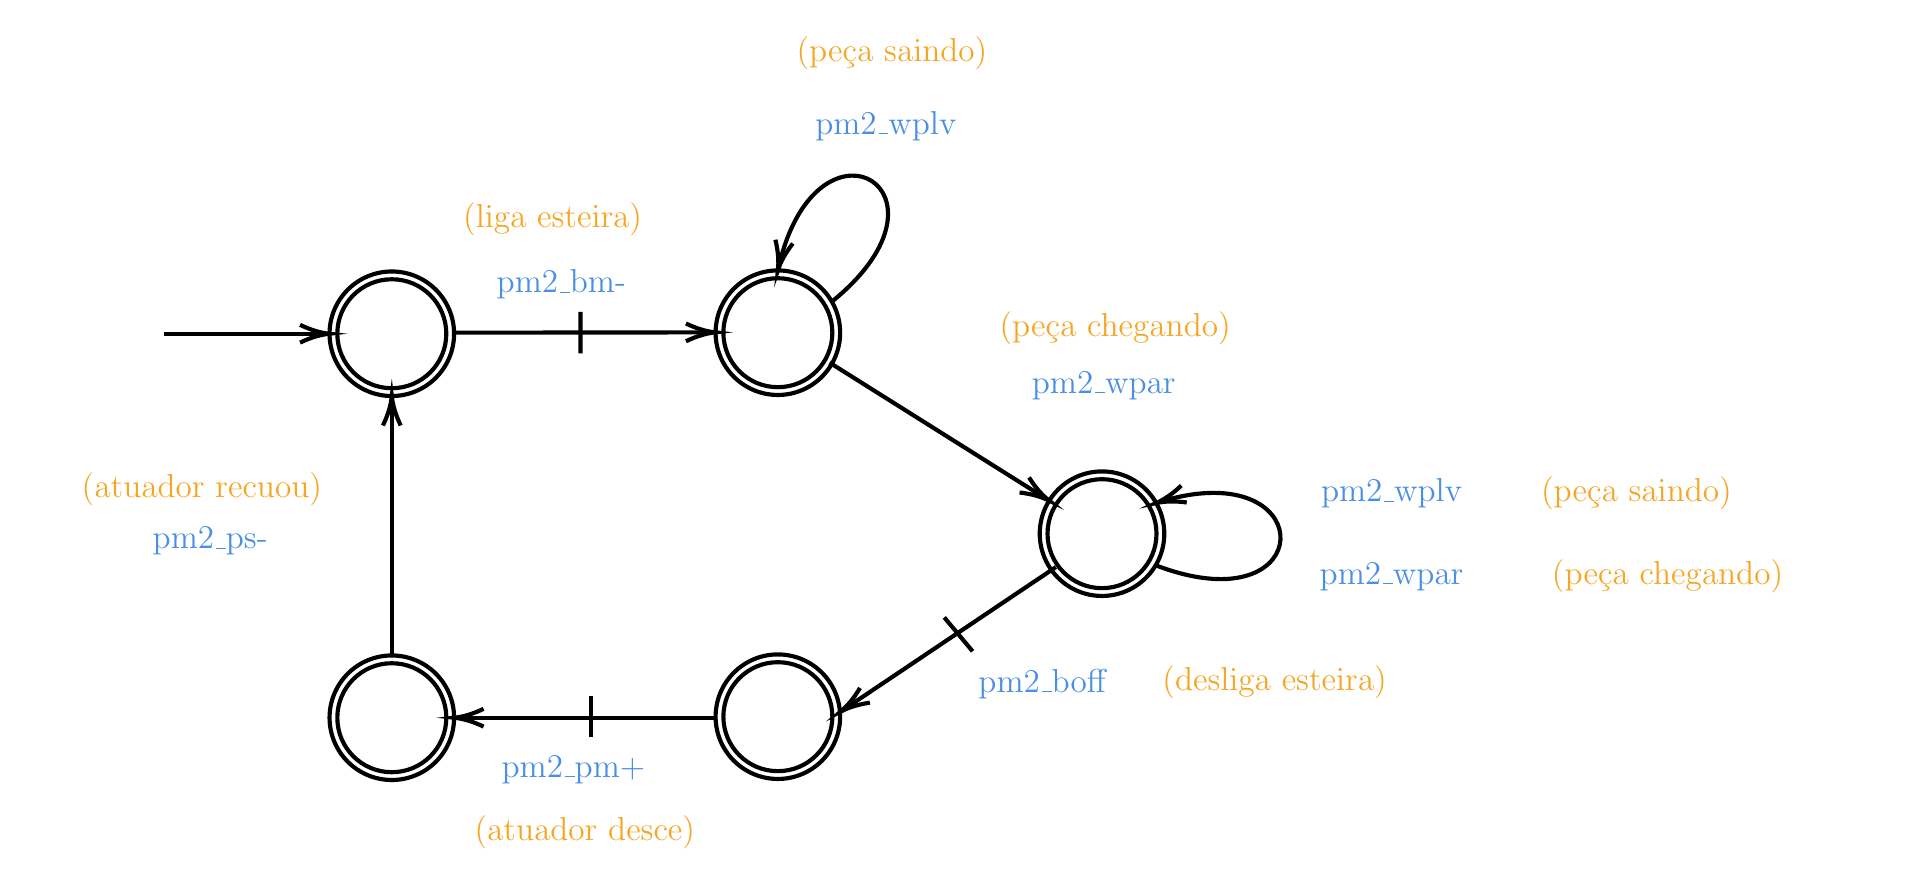
\begin{tikzpicture}[x=0.75pt,y=0.75pt,yscale=-1,xscale=1]
%uncomment if require: \path (0,3420); %set diagram left start at 0, and has height of 3420

%Shape: Circle [id:dp9077579256671899] 
\draw  [line width=1.5]  (1444.5,1540) .. controls (1444.5,1523.43) and (1457.93,1510) .. (1474.5,1510) .. controls (1491.07,1510) and (1504.5,1523.43) .. (1504.5,1540) .. controls (1504.5,1556.57) and (1491.07,1570) .. (1474.5,1570) .. controls (1457.93,1570) and (1444.5,1556.57) .. (1444.5,1540) -- cycle ;
%Shape: Circle [id:dp49050272295100106] 
\draw  [line width=1.5]  (1448.25,1540) .. controls (1448.25,1525.5) and (1460,1513.75) .. (1474.5,1513.75) .. controls (1489,1513.75) and (1500.75,1525.5) .. (1500.75,1540) .. controls (1500.75,1554.5) and (1489,1566.25) .. (1474.5,1566.25) .. controls (1460,1566.25) and (1448.25,1554.5) .. (1448.25,1540) -- cycle ;
%Straight Lines [id:da5069880579739428] 
\draw [line width=1.5]    (1364.5,1540) -- (1441.5,1540) ;
\draw [shift={(1444.5,1540)}, rotate = 180] [color={rgb, 255:red, 0; green, 0; blue, 0 }  ][line width=1.5]    (14.21,-4.28) .. controls (9.04,-1.82) and (4.3,-0.39) .. (0,0) .. controls (4.3,0.39) and (9.04,1.82) .. (14.21,4.28)   ;
%Shape: Circle [id:dp6279882648643924] 
\draw  [line width=1.5]  (1630.5,1539.5) .. controls (1630.5,1522.93) and (1643.93,1509.5) .. (1660.5,1509.5) .. controls (1677.07,1509.5) and (1690.5,1522.93) .. (1690.5,1539.5) .. controls (1690.5,1556.07) and (1677.07,1569.5) .. (1660.5,1569.5) .. controls (1643.93,1569.5) and (1630.5,1556.07) .. (1630.5,1539.5) -- cycle ;
%Straight Lines [id:da9599053460598437] 
\draw [line width=1.5]    (1685.42,1553.91) -- (1704.89,1566.15) -- (1788.71,1618.83) ;
\draw [shift={(1791.25,1620.43)}, rotate = 212.15] [color={rgb, 255:red, 0; green, 0; blue, 0 }  ][line width=1.5]    (14.21,-4.28) .. controls (9.04,-1.82) and (4.3,-0.39) .. (0,0) .. controls (4.3,0.39) and (9.04,1.82) .. (14.21,4.28)   ;
%Straight Lines [id:da49586333480307543] 
\draw [line width=1.5]    (1740.67,1676.67) -- (1754.33,1693) ;
%Shape: Circle [id:dp0045098418455211675] 
\draw  [line width=1.5]  (1630.5,1724.5) .. controls (1630.5,1707.93) and (1643.93,1694.5) .. (1660.5,1694.5) .. controls (1677.07,1694.5) and (1690.5,1707.93) .. (1690.5,1724.5) .. controls (1690.5,1741.07) and (1677.07,1754.5) .. (1660.5,1754.5) .. controls (1643.93,1754.5) and (1630.5,1741.07) .. (1630.5,1724.5) -- cycle ;
%Shape: Circle [id:dp9968433633853042] 
\draw  [line width=1.5]  (1444.5,1725) .. controls (1444.5,1708.43) and (1457.93,1695) .. (1474.5,1695) .. controls (1491.07,1695) and (1504.5,1708.43) .. (1504.5,1725) .. controls (1504.5,1741.57) and (1491.07,1755) .. (1474.5,1755) .. controls (1457.93,1755) and (1444.5,1741.57) .. (1444.5,1725) -- cycle ;
%Straight Lines [id:da3998785728047165] 
\draw [line width=1.5]    (1629.5,1725) -- (1606.5,1725) -- (1507.5,1725) ;
\draw [shift={(1504.5,1725)}, rotate = 360] [color={rgb, 255:red, 0; green, 0; blue, 0 }  ][line width=1.5]    (14.21,-4.28) .. controls (9.04,-1.82) and (4.3,-0.39) .. (0,0) .. controls (4.3,0.39) and (9.04,1.82) .. (14.21,4.28)   ;
%Straight Lines [id:da8755676119075062] 
\draw [line width=1.5]    (1570.5,1734.5) -- (1570.5,1714.5) ;
%Straight Lines [id:da4295420940069248] 
\draw [line width=1.5]    (1474.5,1695) -- (1474.5,1573) ;
\draw [shift={(1474.5,1570)}, rotate = 90] [color={rgb, 255:red, 0; green, 0; blue, 0 }  ][line width=1.5]    (14.21,-4.28) .. controls (9.04,-1.82) and (4.3,-0.39) .. (0,0) .. controls (4.3,0.39) and (9.04,1.82) .. (14.21,4.28)   ;
%Shape: Circle [id:dp9158330958781524] 
\draw  [line width=1.5]  (1634.25,1539.5) .. controls (1634.25,1525) and (1646,1513.25) .. (1660.5,1513.25) .. controls (1675,1513.25) and (1686.75,1525) .. (1686.75,1539.5) .. controls (1686.75,1554) and (1675,1565.75) .. (1660.5,1565.75) .. controls (1646,1565.75) and (1634.25,1554) .. (1634.25,1539.5) -- cycle ;
%Shape: Circle [id:dp9177073337675548] 
\draw  [line width=1.5]  (1448.25,1725) .. controls (1448.25,1710.5) and (1460,1698.75) .. (1474.5,1698.75) .. controls (1489,1698.75) and (1500.75,1710.5) .. (1500.75,1725) .. controls (1500.75,1739.5) and (1489,1751.25) .. (1474.5,1751.25) .. controls (1460,1751.25) and (1448.25,1739.5) .. (1448.25,1725) -- cycle ;
%Shape: Circle [id:dp13905839114905638] 
\draw  [line width=1.5]  (1634.25,1724.5) .. controls (1634.25,1710) and (1646,1698.25) .. (1660.5,1698.25) .. controls (1675,1698.25) and (1686.75,1710) .. (1686.75,1724.5) .. controls (1686.75,1739) and (1675,1750.75) .. (1660.5,1750.75) .. controls (1646,1750.75) and (1634.25,1739) .. (1634.25,1724.5) -- cycle ;
%Shape: Circle [id:dp5145905470381016] 
\draw  [line width=1.5]  (1786.67,1636.33) .. controls (1786.67,1619.76) and (1800.1,1606.33) .. (1816.67,1606.33) .. controls (1833.24,1606.33) and (1846.67,1619.76) .. (1846.67,1636.33) .. controls (1846.67,1652.9) and (1833.24,1666.33) .. (1816.67,1666.33) .. controls (1800.1,1666.33) and (1786.67,1652.9) .. (1786.67,1636.33) -- cycle ;
%Shape: Circle [id:dp43990026803091764] 
\draw  [line width=1.5]  (1790.42,1636.33) .. controls (1790.42,1621.84) and (1802.17,1610.08) .. (1816.67,1610.08) .. controls (1831.16,1610.08) and (1842.92,1621.84) .. (1842.92,1636.33) .. controls (1842.92,1650.83) and (1831.16,1662.58) .. (1816.67,1662.58) .. controls (1802.17,1662.58) and (1790.42,1650.83) .. (1790.42,1636.33) -- cycle ;
%Shape: Boxed Bezier Curve [id:dp1547709151209966] 
\draw [line width=1.5]    (1686.43,1524.6) .. controls (1747.82,1475.02) and (1689.13,1434.17) .. (1665.64,1492.43) .. controls (1663.94,1496.64) and (1662.42,1501.37) .. (1661.15,1506.65) ;
\draw [shift={(1660.5,1509.5)}, rotate = 282.21] [color={rgb, 255:red, 0; green, 0; blue, 0 }  ][line width=1.5]    (14.21,-4.28) .. controls (9.04,-1.82) and (4.3,-0.39) .. (0,0) .. controls (4.3,0.39) and (9.04,1.82) .. (14.21,4.28)   ;
%Shape: Boxed Line [id:dp94520568482204] 
\draw [line width=1.5]    (1794.44,1652.44) -- (1693.15,1720.45) ;
\draw [shift={(1690.66,1722.12)}, rotate = 326.12] [color={rgb, 255:red, 0; green, 0; blue, 0 }  ][line width=1.5]    (14.21,-4.28) .. controls (9.04,-1.82) and (4.3,-0.39) .. (0,0) .. controls (4.3,0.39) and (9.04,1.82) .. (14.21,4.28)   ;
%Shape: Boxed Bezier Curve [id:dp2849664697222474] 
\draw [line width=1.5]    (1842.67,1651.61) .. controls (1916.4,1679.72) and (1922.18,1608.45) .. (1860,1617.46) .. controls (1855.51,1618.11) and (1850.66,1619.18) .. (1845.46,1620.74) ;
\draw [shift={(1842.67,1621.61)}, rotate = 342] [color={rgb, 255:red, 0; green, 0; blue, 0 }  ][line width=1.5]    (14.21,-4.28) .. controls (9.04,-1.82) and (4.3,-0.39) .. (0,0) .. controls (4.3,0.39) and (9.04,1.82) .. (14.21,4.28)   ;
%Straight Lines [id:da30354536494497486] 
\draw [line width=1.5]    (1505.42,1539.48) -- (1528.42,1539.46) -- (1627.42,1539.34) ;
\draw [shift={(1630.42,1539.33)}, rotate = 179.93] [color={rgb, 255:red, 0; green, 0; blue, 0 }  ][line width=1.5]    (14.21,-4.28) .. controls (9.04,-1.82) and (4.3,-0.39) .. (0,0) .. controls (4.3,0.39) and (9.04,1.82) .. (14.21,4.28)   ;
%Straight Lines [id:da805241114651789] 
\draw [line width=1.5]    (1565.4,1529.41) -- (1565.43,1549.41) ;


% Text Node
\draw (1556.17,1516.33) node  [font=\large] [align=left] {\begin{minipage}[lt]{58.23pt}\setlength\topsep{0pt}
\begin{center}
\textcolor[rgb]{0.29,0.56,0.89}{pm2\_bm-}
\end{center}

\end{minipage}};
% Text Node
\draw (1552,1485) node  [font=\large] [align=left] {\begin{minipage}[lt]{119.21pt}\setlength\topsep{0pt}
\begin{center}
\textcolor[rgb]{0.96,0.65,0.14}{(liga esteira)}
\end{center}

\end{minipage}};
% Text Node
\draw (1562,1750) node  [font=\large] [align=left] {\begin{minipage}[lt]{57.55pt}\setlength\topsep{0pt}
\begin{center}
\textcolor[rgb]{0.29,0.56,0.89}{pm2\_pm+}
\end{center}

\end{minipage}};
% Text Node
\draw (1567.5,1780) node  [font=\large] [align=left] {\begin{minipage}[lt]{112.65pt}\setlength\topsep{0pt}
\begin{center}
\textcolor[rgb]{0.96,0.65,0.14}{(atuador desce)}
\end{center}

\end{minipage}};
% Text Node
\draw (1387,1640) node  [font=\large] [align=left] {\begin{minipage}[lt]{57.55pt}\setlength\topsep{0pt}
\begin{center}
\textcolor[rgb]{0.29,0.56,0.89}{pm2\_ps-}
\end{center}

\end{minipage}};
% Text Node
\draw (1383,1615) node  [font=\large] [align=left] {\begin{minipage}[lt]{119.22pt}\setlength\topsep{0pt}
\begin{center}
\textcolor[rgb]{0.96,0.65,0.14}{(atuador recuou)}
\end{center}

\end{minipage}};
% Text Node
\draw (1712.5,1440) node  [font=\large] [align=left] {\begin{minipage}[lt]{58.23pt}\setlength\topsep{0pt}
\begin{center}
\textcolor[rgb]{0.29,0.56,0.89}{pm2\_wplv}
\end{center}

\end{minipage}};
% Text Node
\draw (1715.5,1405) node  [font=\large] [align=left] {\begin{minipage}[lt]{156.17pt}\setlength\topsep{0pt}
\begin{center}
\textcolor[rgb]{0.96,0.65,0.14}{(peça saindo)}
\end{center}

\end{minipage}};
% Text Node
\draw (1817.5,1565) node  [font=\large] [align=left] {\begin{minipage}[lt]{58.23pt}\setlength\topsep{0pt}
\begin{center}
\textcolor[rgb]{0.29,0.56,0.89}{pm2\_wpar}
\end{center}

\end{minipage}};
% Text Node
\draw (1823.01,1537.33) node  [font=\large] [align=left] {\begin{minipage}[lt]{143.25pt}\setlength\topsep{0pt}
\begin{center}
\textcolor[rgb]{0.96,0.65,0.14}{(peça chegando)}
\end{center}

\end{minipage}};
% Text Node
\draw (1787.83,1708.67) node  [font=\large] [align=left] {\begin{minipage}[lt]{58.23pt}\setlength\topsep{0pt}
\begin{center}
\textcolor[rgb]{0.29,0.56,0.89}{pm2\_boff}
\end{center}

\end{minipage}};
% Text Node
\draw (1899.83,1707.67) node  [font=\large] [align=left] {\begin{minipage}[lt]{156.17pt}\setlength\topsep{0pt}
\begin{center}
\textcolor[rgb]{0.96,0.65,0.14}{(desliga esteira)}
\end{center}

\end{minipage}};
% Text Node
\draw (1956.17,1657) node  [font=\large] [align=left] {\begin{minipage}[lt]{58.23pt}\setlength\topsep{0pt}
\begin{center}
\textcolor[rgb]{0.29,0.56,0.89}{pm2\_wpar}
\end{center}

\end{minipage}};
% Text Node
\draw (2089.17,1657) node  [font=\large] [align=left] {\begin{minipage}[lt]{156.17pt}\setlength\topsep{0pt}
\begin{center}
\textcolor[rgb]{0.96,0.65,0.14}{(peça chegando)}
\end{center}

\end{minipage}};
% Text Node
\draw (1956.17,1617) node  [font=\large] [align=left] {\begin{minipage}[lt]{58.23pt}\setlength\topsep{0pt}
\begin{center}
\textcolor[rgb]{0.29,0.56,0.89}{pm2\_wplv}
\end{center}

\end{minipage}};
% Text Node
\draw (2074.17,1617) node  [font=\large] [align=left] {\begin{minipage}[lt]{156.17pt}\setlength\topsep{0pt}
\begin{center}
\textcolor[rgb]{0.96,0.65,0.14}{(peça saindo)}
\end{center}

\end{minipage}};


\end{tikzpicture}}
        \caption{Restrição para PM2.}
        \label{fig:H_PM2}
    \end{figure}


\end{frame}


\begin{frame}{Aplicação do comportamento especificado para cada subsistema.}

    \begin{itemize}
        \item \textbf{Componentes em si não requerem restrições individuais, com exceção da processing machine;} 
        \item \textbf{Utilização de restrições que garantem a interação correta entre diferentes subplantas, garantindo o funcionamento correto.} 
    \end{itemize}

    Subsistemas que requerem restrições:
    \begin{itemize}
        \item \textit{Rotatory Table} e \textit{Processing Machine 1};
        \item \textit{Stack Feeder} e \textit{Exit Slides};
        \item \textit{Rotatory Table} e \textit{Distribution System}.
    \end{itemize}

    

\end{frame}

\begin{frame}{Subplanta \textit{Stack Feeder} (SF) e \textit{Exit Slides} (XSs).}

    Essa restrição é feita para a subplanta contendo \textit{Stack Feeder} e o paralelo entre as duas saídas \textit{Exit Slide}. Tem como objetivo de \textbf{evitar congestionamento} do sistema.

    \begin{figure}[htbp]
        \centering
        \resizebox{0.4\textwidth}{!}{


\tikzset{every picture/.style={line width=0.75pt}} %set default line width to 0.75pt        

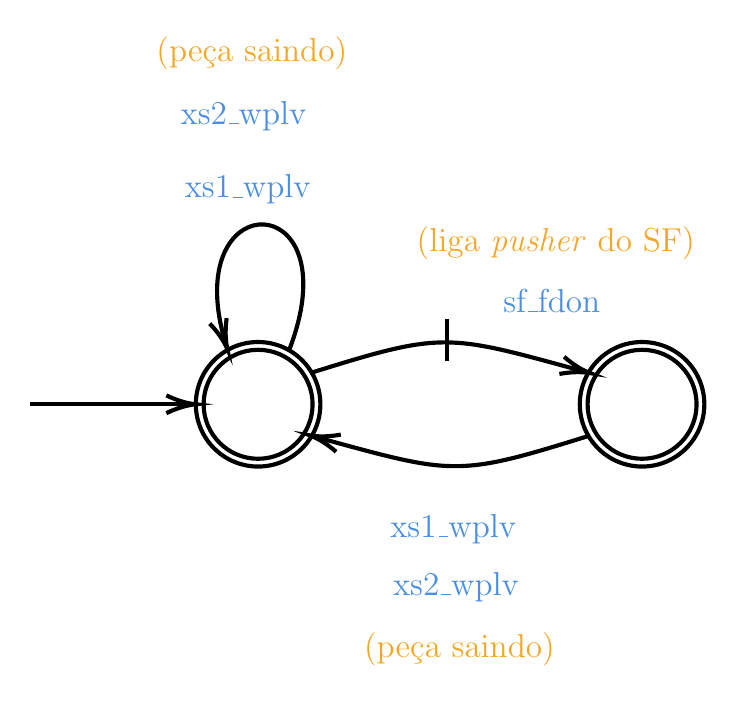
\begin{tikzpicture}[x=0.75pt,y=0.75pt,yscale=-1,xscale=1]
%uncomment if require: \path (0,3420); %set diagram left start at 0, and has height of 3420

%Shape: Circle [id:dp8616914214249671] 
\draw  [line width=1.5]  (1440,404) .. controls (1440,387.43) and (1453.43,374) .. (1470,374) .. controls (1486.57,374) and (1500,387.43) .. (1500,404) .. controls (1500,420.57) and (1486.57,434) .. (1470,434) .. controls (1453.43,434) and (1440,420.57) .. (1440,404) -- cycle ;
%Shape: Circle [id:dp5495288112285035] 
\draw  [line width=1.5]  (1443.75,404) .. controls (1443.75,389.5) and (1455.5,377.75) .. (1470,377.75) .. controls (1484.5,377.75) and (1496.25,389.5) .. (1496.25,404) .. controls (1496.25,418.5) and (1484.5,430.25) .. (1470,430.25) .. controls (1455.5,430.25) and (1443.75,418.5) .. (1443.75,404) -- cycle ;
%Straight Lines [id:da49094404912567957] 
\draw [line width=1.5]    (1360,404) -- (1437,404) ;
\draw [shift={(1440,404)}, rotate = 180] [color={rgb, 255:red, 0; green, 0; blue, 0 }  ][line width=1.5]    (14.21,-4.28) .. controls (9.04,-1.82) and (4.3,-0.39) .. (0,0) .. controls (4.3,0.39) and (9.04,1.82) .. (14.21,4.28)   ;
%Shape: Circle [id:dp8732003190254931] 
\draw  [line width=1.5]  (1625,404) .. controls (1625,387.43) and (1638.43,374) .. (1655,374) .. controls (1671.57,374) and (1685,387.43) .. (1685,404) .. controls (1685,420.57) and (1671.57,434) .. (1655,434) .. controls (1638.43,434) and (1625,420.57) .. (1625,404) -- cycle ;
%Curve Lines [id:da32433354162521333] 
\draw [line width=1.5]    (1495,389) .. controls (1559.85,368.71) and (1560.49,369.97) .. (1627.94,388.44) ;
\draw [shift={(1630,389)}, rotate = 195.29] [color={rgb, 255:red, 0; green, 0; blue, 0 }  ][line width=1.5]    (14.21,-4.28) .. controls (9.04,-1.82) and (4.3,-0.39) .. (0,0) .. controls (4.3,0.39) and (9.04,1.82) .. (14.21,4.28)   ;
%Curve Lines [id:da4326211075777746] 
\draw [line width=1.5]    (1630,419) .. controls (1565.16,439.3) and (1564.51,438.03) .. (1497.06,419.56) ;
\draw [shift={(1495,419)}, rotate = 15.29] [color={rgb, 255:red, 0; green, 0; blue, 0 }  ][line width=1.5]    (14.21,-4.28) .. controls (9.04,-1.82) and (4.3,-0.39) .. (0,0) .. controls (4.3,0.39) and (9.04,1.82) .. (14.21,4.28)   ;
%Shape: Boxed Bezier Curve [id:dp9173651743324984] 
\draw [line width=1.5]    (1485.17,377.33) .. controls (1513.28,303.6) and (1442.01,297.82) .. (1451.02,359.99) .. controls (1451.67,364.49) and (1452.74,369.34) .. (1454.3,374.54) ;
\draw [shift={(1455.17,377.33)}, rotate = 252] [color={rgb, 255:red, 0; green, 0; blue, 0 }  ][line width=1.5]    (14.21,-4.28) .. controls (9.04,-1.82) and (4.3,-0.39) .. (0,0) .. controls (4.3,0.39) and (9.04,1.82) .. (14.21,4.28)   ;
%Straight Lines [id:da8685263968922692] 
\draw [line width=1.5]    (1561,363) -- (1561,383) ;
%Shape: Circle [id:dp2331117907978031] 
\draw  [line width=1.5]  (1628.75,404) .. controls (1628.75,389.5) and (1640.5,377.75) .. (1655,377.75) .. controls (1669.5,377.75) and (1681.25,389.5) .. (1681.25,404) .. controls (1681.25,418.5) and (1669.5,430.25) .. (1655,430.25) .. controls (1640.5,430.25) and (1628.75,418.5) .. (1628.75,404) -- cycle ;

% Text Node
\draw (1611.5,354) node  [font=\large] [align=left] {\begin{minipage}[lt]{51.17pt}\setlength\topsep{0pt}
\begin{center}
\textcolor[rgb]{0.29,0.56,0.89}{sf\_fdon}
\end{center}

\end{minipage}};
% Text Node
\draw (1567,522) node  [font=\large] [align=left] {\begin{minipage}[lt]{91.55pt}\setlength\topsep{0pt}
\begin{center}
\textcolor[rgb]{0.96,0.65,0.14}{(peça saindo)}
\end{center}

\end{minipage}};
% Text Node
\draw (1613.42,326.5) node  [font=\large] [align=left] {\begin{minipage}[lt]{117.75pt}\setlength\topsep{0pt}
\begin{center}
\textcolor[rgb]{0.96,0.65,0.14}{(liga \textit{pusher} do SF)}
\end{center}

\end{minipage}};
% Text Node
\draw (1564,464) node  [font=\large] [align=left] {\begin{minipage}[lt]{51.17pt}\setlength\topsep{0pt}
\begin{center}
\textcolor[rgb]{0.29,0.56,0.89}{xs1\_wplv}
\end{center}

\end{minipage}};
% Text Node
\draw (1465,300.5) node  [font=\large] [align=left] {\begin{minipage}[lt]{51.17pt}\setlength\topsep{0pt}
\begin{center}
\textcolor[rgb]{0.29,0.56,0.89}{xs1\_wplv}
\end{center}

\end{minipage}};
% Text Node
\draw (1467,235) node  [font=\large] [align=left] {\begin{minipage}[lt]{91.55pt}\setlength\topsep{0pt}
\begin{center}
\textcolor[rgb]{0.96,0.65,0.14}{(peça saindo)}
\end{center}

\end{minipage}};
% Text Node
\draw (1463,265) node  [font=\large] [align=left] {\begin{minipage}[lt]{51.17pt}\setlength\topsep{0pt}
\begin{center}
\textcolor[rgb]{0.29,0.56,0.89}{xs2\_wplv}
\end{center}

\end{minipage}};
% Text Node
\draw (1565.33,492) node  [font=\large] [align=left] {\begin{minipage}[lt]{51.17pt}\setlength\topsep{0pt}
\begin{center}
\textcolor[rgb]{0.29,0.56,0.89}{xs2\_wplv}
\end{center}

\end{minipage}};


\end{tikzpicture}}
        \caption{Restrição para SF e XSs.}
        \label{fig:SFXSs}
    \end{figure}
    
\end{frame}

\begin{frame}{Subplanta \textit{Rotatory Table} (RB) e \textit{Processing Machine 1} (PM1).}

    A restrição entre a subplanta contendo \textit{Rotatory Table} e a \textit{Processing Machine 1} e realizada como o paralelo entre duas restrições mais simples.

    \begin{figure}[htbp]
        \centering
        \resizebox{0.7\textwidth}{!}{


\tikzset{every picture/.style={line width=0.75pt}} %set default line width to 0.75pt        

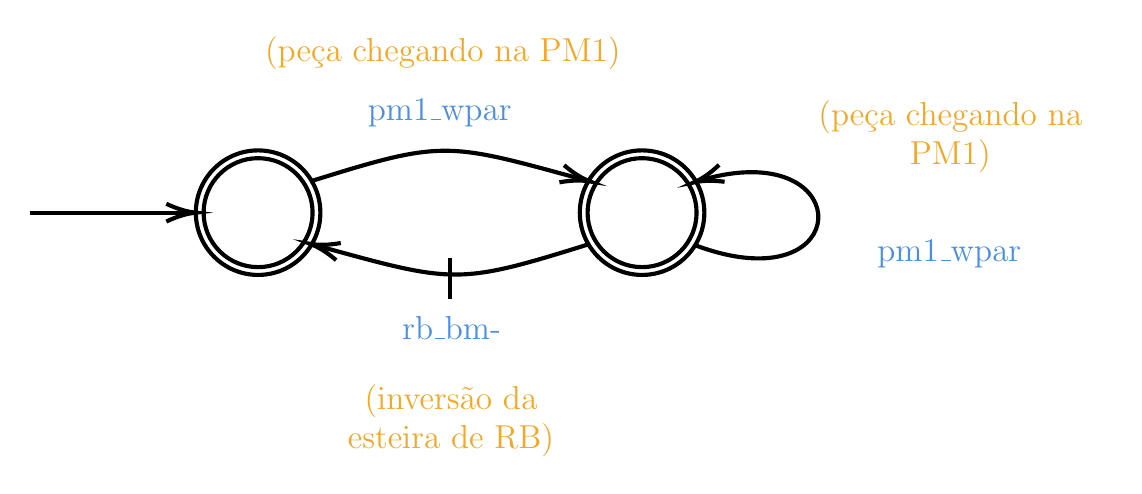
\begin{tikzpicture}[x=0.75pt,y=0.75pt,yscale=-1,xscale=1]
%uncomment if require: \path (0,3420); %set diagram left start at 0, and has height of 3420

%Shape: Circle [id:dp4961981871946022] 
\draw  [line width=1.5]  (1425,1066.67) .. controls (1425,1050.1) and (1438.43,1036.67) .. (1455,1036.67) .. controls (1471.57,1036.67) and (1485,1050.1) .. (1485,1066.67) .. controls (1485,1083.24) and (1471.57,1096.67) .. (1455,1096.67) .. controls (1438.43,1096.67) and (1425,1083.24) .. (1425,1066.67) -- cycle ;
%Shape: Circle [id:dp35043060608825316] 
\draw  [line width=1.5]  (1428.75,1066.67) .. controls (1428.75,1052.17) and (1440.5,1040.42) .. (1455,1040.42) .. controls (1469.5,1040.42) and (1481.25,1052.17) .. (1481.25,1066.67) .. controls (1481.25,1081.16) and (1469.5,1092.92) .. (1455,1092.92) .. controls (1440.5,1092.92) and (1428.75,1081.16) .. (1428.75,1066.67) -- cycle ;
%Straight Lines [id:da27460078941503485] 
\draw [line width=1.5]    (1345,1066.67) -- (1422,1066.67) ;
\draw [shift={(1425,1066.67)}, rotate = 180] [color={rgb, 255:red, 0; green, 0; blue, 0 }  ][line width=1.5]    (14.21,-4.28) .. controls (9.04,-1.82) and (4.3,-0.39) .. (0,0) .. controls (4.3,0.39) and (9.04,1.82) .. (14.21,4.28)   ;
%Shape: Circle [id:dp09618604527762531] 
\draw  [line width=1.5]  (1610,1066.67) .. controls (1610,1050.1) and (1623.43,1036.67) .. (1640,1036.67) .. controls (1656.57,1036.67) and (1670,1050.1) .. (1670,1066.67) .. controls (1670,1083.24) and (1656.57,1096.67) .. (1640,1096.67) .. controls (1623.43,1096.67) and (1610,1083.24) .. (1610,1066.67) -- cycle ;
%Curve Lines [id:da7057273287668866] 
\draw [line width=1.5]    (1480,1051.67) .. controls (1544.85,1031.37) and (1545.49,1032.64) .. (1612.94,1051.1) ;
\draw [shift={(1615,1051.67)}, rotate = 195.29] [color={rgb, 255:red, 0; green, 0; blue, 0 }  ][line width=1.5]    (14.21,-4.28) .. controls (9.04,-1.82) and (4.3,-0.39) .. (0,0) .. controls (4.3,0.39) and (9.04,1.82) .. (14.21,4.28)   ;
%Curve Lines [id:da02333708563685888] 
\draw [line width=1.5]    (1615,1081.67) .. controls (1550.16,1101.96) and (1549.51,1100.69) .. (1482.06,1082.23) ;
\draw [shift={(1480,1081.67)}, rotate = 15.29] [color={rgb, 255:red, 0; green, 0; blue, 0 }  ][line width=1.5]    (14.21,-4.28) .. controls (9.04,-1.82) and (4.3,-0.39) .. (0,0) .. controls (4.3,0.39) and (9.04,1.82) .. (14.21,4.28)   ;
%Shape: Boxed Bezier Curve [id:dp5607023531802633] 
\draw [line width=1.5]    (1664.92,1082.11) .. controls (1738.65,1110.22) and (1744.43,1038.95) .. (1682.26,1047.96) .. controls (1677.76,1048.61) and (1672.91,1049.68) .. (1667.71,1051.24) ;
\draw [shift={(1664.92,1052.11)}, rotate = 342] [color={rgb, 255:red, 0; green, 0; blue, 0 }  ][line width=1.5]    (14.21,-4.28) .. controls (9.04,-1.82) and (4.3,-0.39) .. (0,0) .. controls (4.3,0.39) and (9.04,1.82) .. (14.21,4.28)   ;
%Straight Lines [id:da4120300873361482] 
\draw [line width=1.5]    (1547.33,1088.33) -- (1547.33,1108.33) ;
%Shape: Circle [id:dp6932255437272121] 
\draw  [line width=1.5]  (1613.75,1066.67) .. controls (1613.75,1052.17) and (1625.5,1040.42) .. (1640,1040.42) .. controls (1654.5,1040.42) and (1666.25,1052.17) .. (1666.25,1066.67) .. controls (1666.25,1081.16) and (1654.5,1092.92) .. (1640,1092.92) .. controls (1625.5,1092.92) and (1613.75,1081.16) .. (1613.75,1066.67) -- cycle ;

% Text Node
\draw (1542.5,1018.5) node  [font=\large] [align=left] {\begin{minipage}[lt]{69.05pt}\setlength\topsep{0pt}
\begin{center}
\textcolor[rgb]{0.29,0.56,0.89}{pm1\_wpar}
\end{center}

\end{minipage}};
% Text Node
\draw (1547.92,1166.79) node  [font=\large] [align=left] {\begin{minipage}[lt]{91.55pt}\setlength\topsep{0pt}
\begin{center}
\textcolor[rgb]{0.96,0.65,0.14}{(inversão da esteira de RB)}
\end{center}

\end{minipage}};
% Text Node
\draw (1548.26,1122.17) node  [font=\large] [align=left] {\begin{minipage}[lt]{51.17pt}\setlength\topsep{0pt}
\begin{center}
\textcolor[rgb]{0.29,0.56,0.89}{rb\_bm-}
\end{center}

\end{minipage}};
% Text Node
\draw (1788.5,1030) node  [font=\large] [align=left] {\begin{minipage}[lt]{111.73pt}\setlength\topsep{0pt}
\begin{center}
\textcolor[rgb]{0.96,0.65,0.14}{(peça chegando na PM1)}
\end{center}

\end{minipage}};
% Text Node
\draw (1544,990) node  [font=\large] [align=left] {\begin{minipage}[lt]{148.69pt}\setlength\topsep{0pt}
\begin{center}
\textcolor[rgb]{0.96,0.65,0.14}{(peça chegando na PM1)}
\end{center}

\end{minipage}};
% Text Node
\draw (1788,1086.5) node  [font=\large] [align=left] {\begin{minipage}[lt]{69.05pt}\setlength\topsep{0pt}
\begin{center}
\textcolor[rgb]{0.29,0.56,0.89}{pm1\_wpar}
\end{center}

\end{minipage}};


\end{tikzpicture}}
        \caption{\textbf{Primeira} restrição para RB e PM1 (controle da inversão do sentido da esteira de RB).}
        \label{fig:SFXSs} 
    \end{figure}
    
\end{frame}

\begin{frame}{Subplanta \textit{Rotatory Table} (RB) e \textit{Processing Machine 1} (PM1).}

    \begin{figure}[htbp]
        \centering
        \resizebox{0.75\textwidth}{!}{


\tikzset{every picture/.style={line width=0.75pt}} %set default line width to 0.75pt        

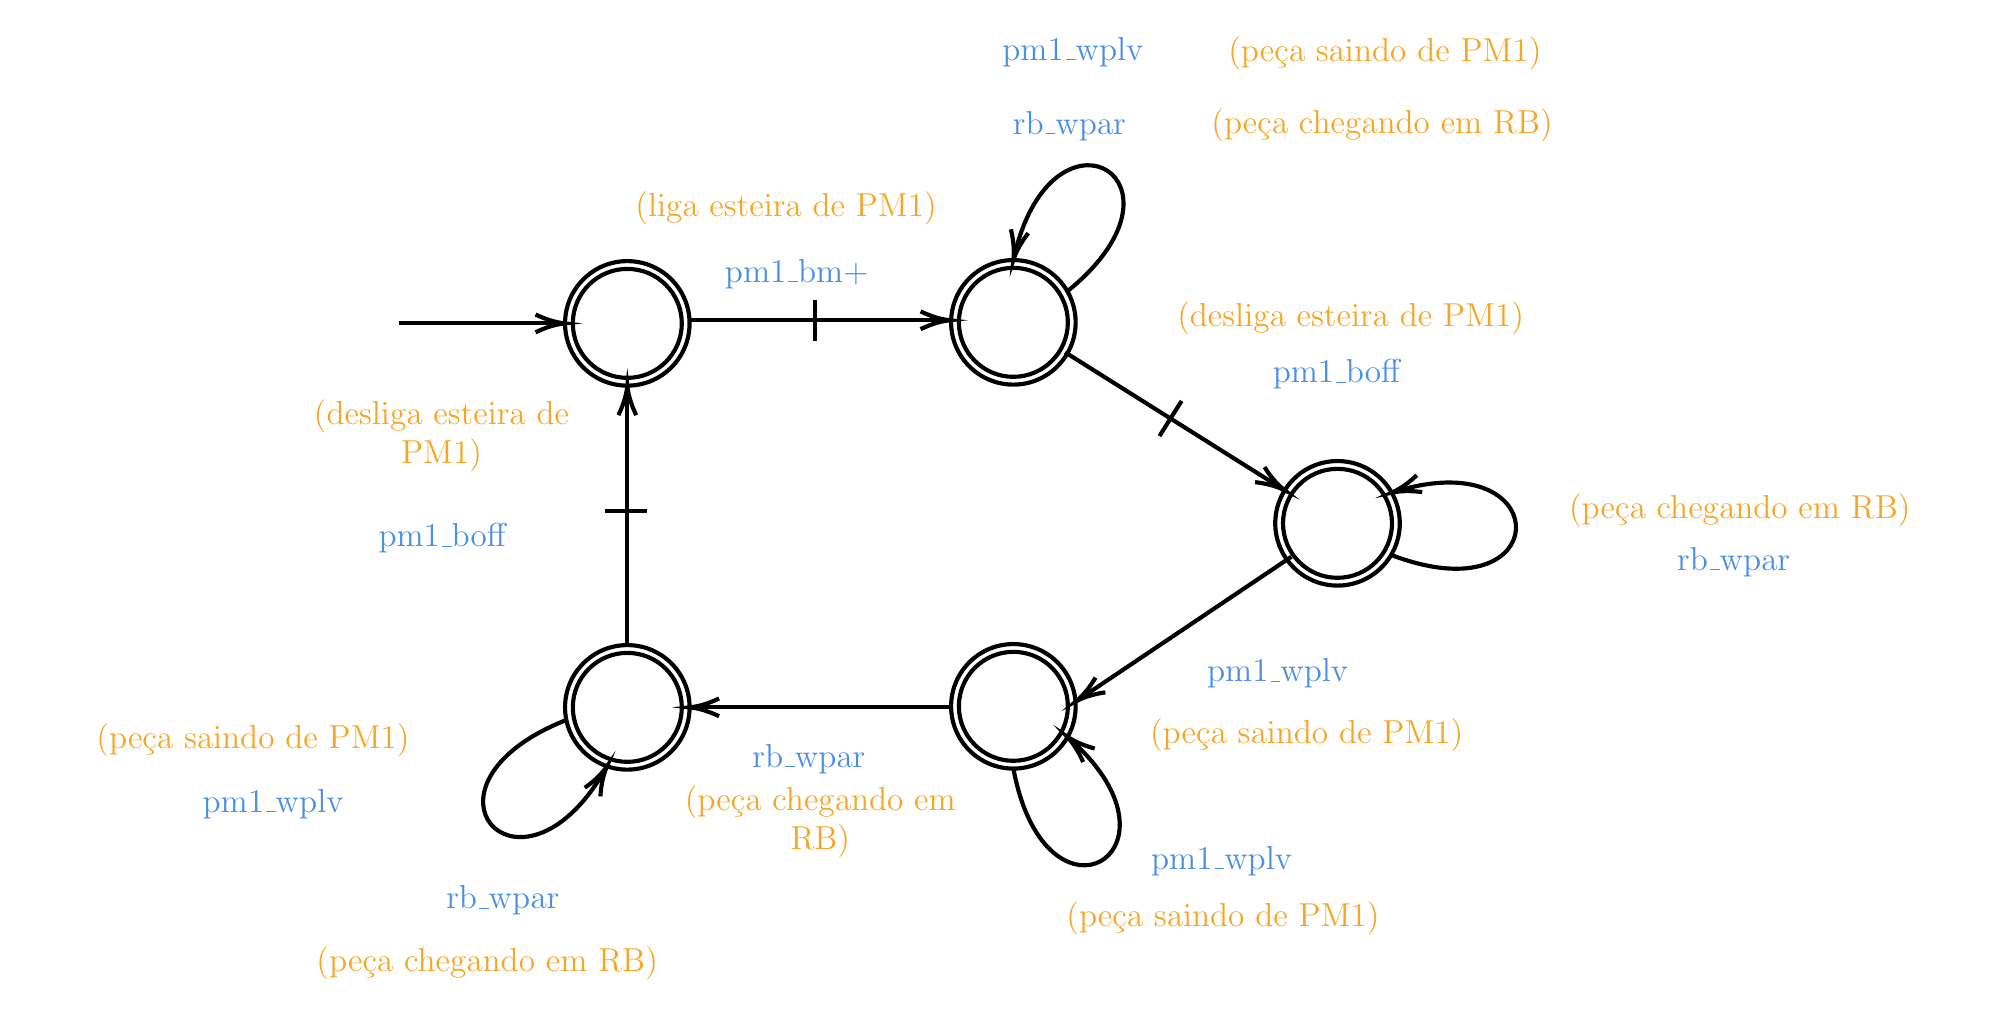
\begin{tikzpicture}[x=0.75pt,y=0.75pt,yscale=-1,xscale=1]
%uncomment if require: \path (0,3420); %set diagram left start at 0, and has height of 3420

%Shape: Circle [id:dp23601440540319296] 
\draw  [line width=1.5]  (1669.5,2181.5) .. controls (1669.5,2164.93) and (1682.93,2151.5) .. (1699.5,2151.5) .. controls (1716.07,2151.5) and (1729.5,2164.93) .. (1729.5,2181.5) .. controls (1729.5,2198.07) and (1716.07,2211.5) .. (1699.5,2211.5) .. controls (1682.93,2211.5) and (1669.5,2198.07) .. (1669.5,2181.5) -- cycle ;
%Shape: Circle [id:dp2022980675381547] 
\draw  [line width=1.5]  (1673.25,2181.5) .. controls (1673.25,2167) and (1685,2155.25) .. (1699.5,2155.25) .. controls (1714,2155.25) and (1725.75,2167) .. (1725.75,2181.5) .. controls (1725.75,2196) and (1714,2207.75) .. (1699.5,2207.75) .. controls (1685,2207.75) and (1673.25,2196) .. (1673.25,2181.5) -- cycle ;
%Straight Lines [id:da20360687176649162] 
\draw [line width=1.5]    (1589.5,2181.5) -- (1666.5,2181.5) ;
\draw [shift={(1669.5,2181.5)}, rotate = 180] [color={rgb, 255:red, 0; green, 0; blue, 0 }  ][line width=1.5]    (14.21,-4.28) .. controls (9.04,-1.82) and (4.3,-0.39) .. (0,0) .. controls (4.3,0.39) and (9.04,1.82) .. (14.21,4.28)   ;
%Shape: Circle [id:dp5581776719780993] 
\draw  [line width=1.5]  (1855.5,2181) .. controls (1855.5,2164.43) and (1868.93,2151) .. (1885.5,2151) .. controls (1902.07,2151) and (1915.5,2164.43) .. (1915.5,2181) .. controls (1915.5,2197.57) and (1902.07,2211) .. (1885.5,2211) .. controls (1868.93,2211) and (1855.5,2197.57) .. (1855.5,2181) -- cycle ;
%Straight Lines [id:da6469225581898377] 
\draw [line width=1.5]    (1910.42,2195.41) -- (1929.89,2207.65) -- (2013.71,2260.33) ;
\draw [shift={(2016.25,2261.93)}, rotate = 212.15] [color={rgb, 255:red, 0; green, 0; blue, 0 }  ][line width=1.5]    (14.21,-4.28) .. controls (9.04,-1.82) and (4.3,-0.39) .. (0,0) .. controls (4.3,0.39) and (9.04,1.82) .. (14.21,4.28)   ;
%Straight Lines [id:da9071024479041658] 
\draw [line width=1.5]    (1966.54,2218.87) -- (1955.9,2235.8) ;

%Shape: Circle [id:dp40872647102696935] 
\draw  [line width=1.5]  (1855.5,2366) .. controls (1855.5,2349.43) and (1868.93,2336) .. (1885.5,2336) .. controls (1902.07,2336) and (1915.5,2349.43) .. (1915.5,2366) .. controls (1915.5,2382.57) and (1902.07,2396) .. (1885.5,2396) .. controls (1868.93,2396) and (1855.5,2382.57) .. (1855.5,2366) -- cycle ;
%Shape: Circle [id:dp5565476487030998] 
\draw  [line width=1.5]  (1669.5,2366.5) .. controls (1669.5,2349.93) and (1682.93,2336.5) .. (1699.5,2336.5) .. controls (1716.07,2336.5) and (1729.5,2349.93) .. (1729.5,2366.5) .. controls (1729.5,2383.07) and (1716.07,2396.5) .. (1699.5,2396.5) .. controls (1682.93,2396.5) and (1669.5,2383.07) .. (1669.5,2366.5) -- cycle ;
%Straight Lines [id:da9239255372434181] 
\draw [line width=1.5]    (1854.5,2366.5) -- (1831.5,2366.5) -- (1732.5,2366.5) ;
\draw [shift={(1729.5,2366.5)}, rotate = 360] [color={rgb, 255:red, 0; green, 0; blue, 0 }  ][line width=1.5]    (14.21,-4.28) .. controls (9.04,-1.82) and (4.3,-0.39) .. (0,0) .. controls (4.3,0.39) and (9.04,1.82) .. (14.21,4.28)   ;
%Straight Lines [id:da8733738548126078] 
\draw [line width=1.5]    (1708.9,2272) -- (1688.9,2272) ;
%Shape: Boxed Line [id:dp4537179801660236] 
\draw [line width=1.5]    (1699.5,2336.5) -- (1699.5,2214.5) ;
\draw [shift={(1699.5,2211.5)}, rotate = 90] [color={rgb, 255:red, 0; green, 0; blue, 0 }  ][line width=1.5]    (14.21,-4.28) .. controls (9.04,-1.82) and (4.3,-0.39) .. (0,0) .. controls (4.3,0.39) and (9.04,1.82) .. (14.21,4.28)   ;
%Shape: Circle [id:dp4448293272065569] 
\draw  [line width=1.5]  (1859.25,2181) .. controls (1859.25,2166.5) and (1871,2154.75) .. (1885.5,2154.75) .. controls (1900,2154.75) and (1911.75,2166.5) .. (1911.75,2181) .. controls (1911.75,2195.5) and (1900,2207.25) .. (1885.5,2207.25) .. controls (1871,2207.25) and (1859.25,2195.5) .. (1859.25,2181) -- cycle ;
%Shape: Circle [id:dp7597357964705245] 
\draw  [line width=1.5]  (1673.25,2366.5) .. controls (1673.25,2352) and (1685,2340.25) .. (1699.5,2340.25) .. controls (1714,2340.25) and (1725.75,2352) .. (1725.75,2366.5) .. controls (1725.75,2381) and (1714,2392.75) .. (1699.5,2392.75) .. controls (1685,2392.75) and (1673.25,2381) .. (1673.25,2366.5) -- cycle ;
%Shape: Circle [id:dp8656429564666801] 
\draw  [line width=1.5]  (1859.25,2366) .. controls (1859.25,2351.5) and (1871,2339.75) .. (1885.5,2339.75) .. controls (1900,2339.75) and (1911.75,2351.5) .. (1911.75,2366) .. controls (1911.75,2380.5) and (1900,2392.25) .. (1885.5,2392.25) .. controls (1871,2392.25) and (1859.25,2380.5) .. (1859.25,2366) -- cycle ;
%Shape: Circle [id:dp3733710350679478] 
\draw  [line width=1.5]  (2011.67,2277.83) .. controls (2011.67,2261.26) and (2025.1,2247.83) .. (2041.67,2247.83) .. controls (2058.24,2247.83) and (2071.67,2261.26) .. (2071.67,2277.83) .. controls (2071.67,2294.4) and (2058.24,2307.83) .. (2041.67,2307.83) .. controls (2025.1,2307.83) and (2011.67,2294.4) .. (2011.67,2277.83) -- cycle ;
%Shape: Circle [id:dp8182020576096669] 
\draw  [line width=1.5]  (2015.42,2277.83) .. controls (2015.42,2263.34) and (2027.17,2251.58) .. (2041.67,2251.58) .. controls (2056.16,2251.58) and (2067.92,2263.34) .. (2067.92,2277.83) .. controls (2067.92,2292.33) and (2056.16,2304.08) .. (2041.67,2304.08) .. controls (2027.17,2304.08) and (2015.42,2292.33) .. (2015.42,2277.83) -- cycle ;
%Shape: Boxed Bezier Curve [id:dp5547457937556954] 
\draw [line width=1.5]    (1911.43,2166.1) .. controls (1972.82,2116.52) and (1914.13,2075.67) .. (1890.64,2133.93) .. controls (1888.94,2138.14) and (1887.42,2142.87) .. (1886.15,2148.15) ;
\draw [shift={(1885.5,2151)}, rotate = 282.21] [color={rgb, 255:red, 0; green, 0; blue, 0 }  ][line width=1.5]    (14.21,-4.28) .. controls (9.04,-1.82) and (4.3,-0.39) .. (0,0) .. controls (4.3,0.39) and (9.04,1.82) .. (14.21,4.28)   ;
%Shape: Boxed Line [id:dp33908331846833417] 
\draw [line width=1.5]    (2019.44,2293.94) -- (1918.15,2361.95) ;
\draw [shift={(1915.66,2363.62)}, rotate = 326.12] [color={rgb, 255:red, 0; green, 0; blue, 0 }  ][line width=1.5]    (14.21,-4.28) .. controls (9.04,-1.82) and (4.3,-0.39) .. (0,0) .. controls (4.3,0.39) and (9.04,1.82) .. (14.21,4.28)   ;
%Shape: Boxed Bezier Curve [id:dp3416016771200352] 
\draw [line width=1.5]    (2067.67,2293.11) .. controls (2141.4,2321.22) and (2147.18,2249.95) .. (2085,2258.96) .. controls (2080.51,2259.61) and (2075.66,2260.68) .. (2070.46,2262.24) ;
\draw [shift={(2067.67,2263.11)}, rotate = 342] [color={rgb, 255:red, 0; green, 0; blue, 0 }  ][line width=1.5]    (14.21,-4.28) .. controls (9.04,-1.82) and (4.3,-0.39) .. (0,0) .. controls (4.3,0.39) and (9.04,1.82) .. (14.21,4.28)   ;
%Shape: Boxed Bezier Curve [id:dp4418114948340497] 
\draw [line width=1.5]    (1885.5,2396) .. controls (1900.02,2473.56) and (1963.82,2441.28) .. (1923.68,2392.96) .. controls (1920.78,2389.47) and (1917.33,2385.89) .. (1913.29,2382.26) ;
\draw [shift={(1911.09,2380.34)}, rotate = 40.53] [color={rgb, 255:red, 0; green, 0; blue, 0 }  ][line width=1.5]    (14.21,-4.28) .. controls (9.04,-1.82) and (4.3,-0.39) .. (0,0) .. controls (4.3,0.39) and (9.04,1.82) .. (14.21,4.28)   ;
%Shape: Boxed Bezier Curve [id:dp3570860014303048] 
\draw [line width=1.5]    (1669.29,2372.91) .. controls (1596.13,2402.47) and (1640.38,2458.64) .. (1679.82,2409.74) .. controls (1682.67,2406.2) and (1685.49,2402.12) .. (1688.25,2397.43) ;
\draw [shift={(1689.7,2394.9)}, rotate = 119.13] [color={rgb, 255:red, 0; green, 0; blue, 0 }  ][line width=1.5]    (14.21,-4.28) .. controls (9.04,-1.82) and (4.3,-0.39) .. (0,0) .. controls (4.3,0.39) and (9.04,1.82) .. (14.21,4.28)   ;
%Straight Lines [id:da1195292766490681] 
\draw [line width=1.5]    (1730,2180) -- (1753,2180) -- (1852,2180) ;
\draw [shift={(1855,2180)}, rotate = 180] [color={rgb, 255:red, 0; green, 0; blue, 0 }  ][line width=1.5]    (14.21,-4.28) .. controls (9.04,-1.82) and (4.3,-0.39) .. (0,0) .. controls (4.3,0.39) and (9.04,1.82) .. (14.21,4.28)   ;
%Straight Lines [id:da8661652565645079] 
\draw [line width=1.5]    (1790,2170) -- (1790,2190) ;


% Text Node
\draw (1781.17,2157.83) node  [font=\large] [align=left] {\begin{minipage}[lt]{58.23pt}\setlength\topsep{0pt}
\begin{center}
\textcolor[rgb]{0.29,0.56,0.89}{pm1\_bm+}
\end{center}

\end{minipage}};
% Text Node
\draw (1776.01,2126) node  [font=\large] [align=left] {\begin{minipage}[lt]{119.21pt}\setlength\topsep{0pt}
\begin{center}
\textcolor[rgb]{0.96,0.65,0.14}{(liga esteira de PM1)}
\end{center}

\end{minipage}};
% Text Node
\draw (1787,2391.5) node  [font=\large] [align=left] {\begin{minipage}[lt]{57.55pt}\setlength\topsep{0pt}
\begin{center}
\textcolor[rgb]{0.29,0.56,0.89}{rb\_wpar}
\end{center}

\end{minipage}};
% Text Node
\draw (1792.5,2421.5) node  [font=\large] [align=left] {\begin{minipage}[lt]{112.65pt}\setlength\topsep{0pt}
\begin{center}
\textcolor[rgb]{0.96,0.65,0.14}{(peça chegando em RB)}
\end{center}

\end{minipage}};
% Text Node
\draw (1610.33,2285.17) node  [font=\large] [align=left] {\begin{minipage}[lt]{57.55pt}\setlength\topsep{0pt}
\begin{center}
\textcolor[rgb]{0.29,0.56,0.89}{pm1\_boff}
\end{center}

\end{minipage}};
% Text Node
\draw (1610,2235.5) node  [font=\large] [align=left] {\begin{minipage}[lt]{119.22pt}\setlength\topsep{0pt}
\begin{center}
\textcolor[rgb]{0.96,0.65,0.14}{(desliga esteira de PM1)}
\end{center}

\end{minipage}};
% Text Node
\draw (1914.17,2050.83) node  [font=\large] [align=left] {\begin{minipage}[lt]{58.23pt}\setlength\topsep{0pt}
\begin{center}
\textcolor[rgb]{0.29,0.56,0.89}{pm1\_wplv}
\end{center}

\end{minipage}};
% Text Node
\draw (2064.5,2051.5) node  [font=\large] [align=left] {\begin{minipage}[lt]{156.17pt}\setlength\topsep{0pt}
\begin{center}
\textcolor[rgb]{0.96,0.65,0.14}{(peça saindo de PM1)}
\end{center}

\end{minipage}};
% Text Node
\draw (1912.5,2086.5) node  [font=\large] [align=left] {\begin{minipage}[lt]{58.23pt}\setlength\topsep{0pt}
\begin{center}
\textcolor[rgb]{0.29,0.56,0.89}{rb\_wpar}
\end{center}

\end{minipage}};
% Text Node
\draw (2063.17,2085.83) node  [font=\large] [align=left] {\begin{minipage}[lt]{156.17pt}\setlength\topsep{0pt}
\begin{center}
\textcolor[rgb]{0.96,0.65,0.14}{(peça chegando em RB)}
\end{center}

\end{minipage}};
% Text Node
\draw (2041.17,2206.17) node  [font=\large] [align=left] {\begin{minipage}[lt]{58.23pt}\setlength\topsep{0pt}
\begin{center}
\textcolor[rgb]{0.29,0.56,0.89}{pm1\_boff}
\end{center}

\end{minipage}};
% Text Node
\draw (2048.01,2178.83) node  [font=\large] [align=left] {\begin{minipage}[lt]{143.25pt}\setlength\topsep{0pt}
\begin{center}
\textcolor[rgb]{0.96,0.65,0.14}{(desliga esteira de PM1)}
\end{center}

\end{minipage}};
% Text Node
\draw (2012.83,2350.17) node  [font=\large] [align=left] {\begin{minipage}[lt]{58.23pt}\setlength\topsep{0pt}
\begin{center}
\textcolor[rgb]{0.29,0.56,0.89}{pm1\_wplv}
\end{center}

\end{minipage}};
% Text Node
\draw (2026.83,2379.83) node  [font=\large] [align=left] {\begin{minipage}[lt]{156.17pt}\setlength\topsep{0pt}
\begin{center}
\textcolor[rgb]{0.96,0.65,0.14}{(peça saindo de PM1)}
\end{center}

\end{minipage}};
% Text Node
\draw (2232.5,2296.5) node  [font=\large] [align=left] {\begin{minipage}[lt]{58.23pt}\setlength\topsep{0pt}
\begin{center}
\textcolor[rgb]{0.29,0.56,0.89}{rb\_wpar}
\end{center}

\end{minipage}};
% Text Node
\draw (2235.5,2271.5) node  [font=\large] [align=left] {\begin{minipage}[lt]{156.17pt}\setlength\topsep{0pt}
\begin{center}
\textcolor[rgb]{0.96,0.65,0.14}{(peça chegando em RB)}
\end{center}

\end{minipage}};
% Text Node
\draw (1985.83,2440.5) node  [font=\large] [align=left] {\begin{minipage}[lt]{58.23pt}\setlength\topsep{0pt}
\begin{center}
\textcolor[rgb]{0.29,0.56,0.89}{pm1\_wplv}
\end{center}

\end{minipage}};
% Text Node
\draw (1986.5,2468.17) node  [font=\large] [align=left] {\begin{minipage}[lt]{156.17pt}\setlength\topsep{0pt}
\begin{center}
\textcolor[rgb]{0.96,0.65,0.14}{(peça saindo de PM1)}
\end{center}

\end{minipage}};
% Text Node
\draw (1528.83,2413.17) node  [font=\large] [align=left] {\begin{minipage}[lt]{58.23pt}\setlength\topsep{0pt}
\begin{center}
\textcolor[rgb]{0.29,0.56,0.89}{pm1\_wplv}
\end{center}

\end{minipage}};
% Text Node
\draw (1519.17,2382.5) node  [font=\large] [align=left] {\begin{minipage}[lt]{156.17pt}\setlength\topsep{0pt}
\begin{center}
\textcolor[rgb]{0.96,0.65,0.14}{(peça saindo de PM1)}
\end{center}

\end{minipage}};
% Text Node
\draw (1639.5,2459.5) node  [font=\large] [align=left] {\begin{minipage}[lt]{58.23pt}\setlength\topsep{0pt}
\begin{center}
\textcolor[rgb]{0.29,0.56,0.89}{rb\_wpar}
\end{center}

\end{minipage}};
% Text Node
\draw (1632,2490) node  [font=\large] [align=left] {\begin{minipage}[lt]{156.17pt}\setlength\topsep{0pt}
\begin{center}
\textcolor[rgb]{0.96,0.65,0.14}{(peça chegando em RB)}
\end{center}

\end{minipage}};


\end{tikzpicture}}
        \caption{\textbf{Segunda} restrição para RB e PM1 (controle da ordem de funcionamento da esteira de PM1).}
        \label{fig:SFXSs} 
    \end{figure}
    
\end{frame}

\begin{frame}{Subplanta \textit{Rotatory Table} (RB) e \textit{Distribution System} (DS).}

    Essa restrição é feita para a subplanta contendo \textit{Rotatory Table} e o \textit{Distribution System}.

    \begin{figure}[htbp]
        \centering
        \resizebox{0.8\textwidth}{!}{


\tikzset{every picture/.style={line width=0.75pt}} %set default line width to 0.75pt        

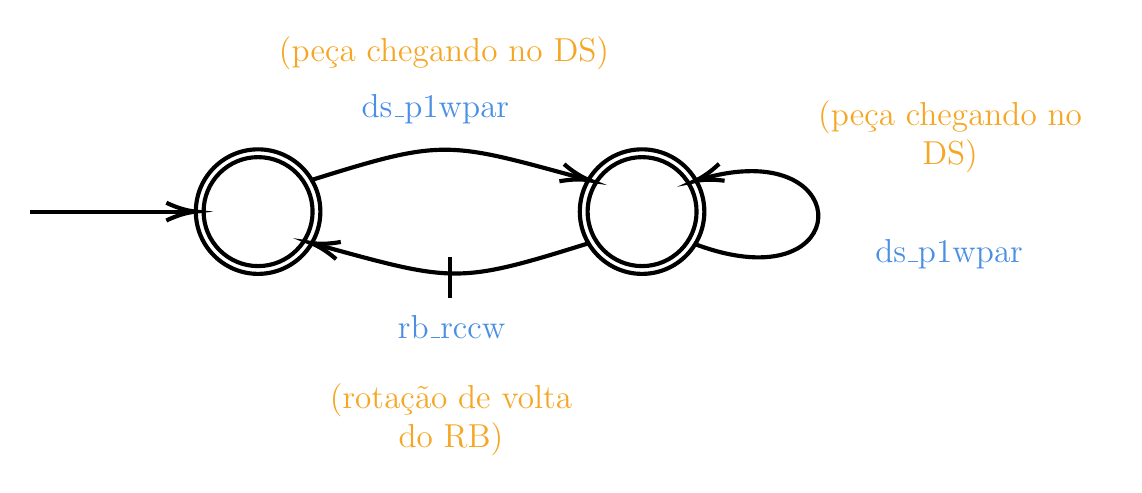
\begin{tikzpicture}[x=0.75pt,y=0.75pt,yscale=-1,xscale=1]
%uncomment if require: \path (0,3420); %set diagram left start at 0, and has height of 3420

%Shape: Circle [id:dp8461873664121] 
\draw  [line width=1.5]  (1425.08,774.5) .. controls (1425.08,757.93) and (1438.51,744.5) .. (1455.08,744.5) .. controls (1471.65,744.5) and (1485.08,757.93) .. (1485.08,774.5) .. controls (1485.08,791.07) and (1471.65,804.5) .. (1455.08,804.5) .. controls (1438.51,804.5) and (1425.08,791.07) .. (1425.08,774.5) -- cycle ;
%Shape: Circle [id:dp46270913419843795] 
\draw  [line width=1.5]  (1428.83,774.5) .. controls (1428.83,760) and (1440.58,748.25) .. (1455.08,748.25) .. controls (1469.58,748.25) and (1481.33,760) .. (1481.33,774.5) .. controls (1481.33,789) and (1469.58,800.75) .. (1455.08,800.75) .. controls (1440.58,800.75) and (1428.83,789) .. (1428.83,774.5) -- cycle ;
%Straight Lines [id:da7878026251103061] 
\draw [line width=1.5]    (1345.08,774.5) -- (1422.08,774.5) ;
\draw [shift={(1425.08,774.5)}, rotate = 180] [color={rgb, 255:red, 0; green, 0; blue, 0 }  ][line width=1.5]    (14.21,-4.28) .. controls (9.04,-1.82) and (4.3,-0.39) .. (0,0) .. controls (4.3,0.39) and (9.04,1.82) .. (14.21,4.28)   ;
%Shape: Circle [id:dp5561173192775071] 
\draw  [line width=1.5]  (1610.08,774.5) .. controls (1610.08,757.93) and (1623.51,744.5) .. (1640.08,744.5) .. controls (1656.65,744.5) and (1670.08,757.93) .. (1670.08,774.5) .. controls (1670.08,791.07) and (1656.65,804.5) .. (1640.08,804.5) .. controls (1623.51,804.5) and (1610.08,791.07) .. (1610.08,774.5) -- cycle ;
%Curve Lines [id:da005002173928317921] 
\draw [line width=1.5]    (1480.08,759.5) .. controls (1544.92,739.21) and (1545.57,740.47) .. (1613.01,758.94) ;
\draw [shift={(1615.08,759.5)}, rotate = 195.29] [color={rgb, 255:red, 0; green, 0; blue, 0 }  ][line width=1.5]    (14.21,-4.28) .. controls (9.04,-1.82) and (4.3,-0.39) .. (0,0) .. controls (4.3,0.39) and (9.04,1.82) .. (14.21,4.28)   ;
%Curve Lines [id:da7416910169510444] 
\draw [line width=1.5]    (1615.08,789.5) .. controls (1550.23,809.8) and (1549.58,808.53) .. (1482.14,790.06) ;
\draw [shift={(1480.08,789.5)}, rotate = 15.29] [color={rgb, 255:red, 0; green, 0; blue, 0 }  ][line width=1.5]    (14.21,-4.28) .. controls (9.04,-1.82) and (4.3,-0.39) .. (0,0) .. controls (4.3,0.39) and (9.04,1.82) .. (14.21,4.28)   ;
%Shape: Boxed Bezier Curve [id:dp610073700876802] 
\draw [line width=1.5]    (1665,789.94) .. controls (1738.73,818.05) and (1744.51,746.79) .. (1682.34,755.79) .. controls (1677.84,756.44) and (1672.99,757.52) .. (1667.79,759.07) ;
\draw [shift={(1665,759.94)}, rotate = 342] [color={rgb, 255:red, 0; green, 0; blue, 0 }  ][line width=1.5]    (14.21,-4.28) .. controls (9.04,-1.82) and (4.3,-0.39) .. (0,0) .. controls (4.3,0.39) and (9.04,1.82) .. (14.21,4.28)   ;
%Straight Lines [id:da2855003368533755] 
\draw [line width=1.5]    (1547.41,796.17) -- (1547.41,816.17) ;
%Shape: Circle [id:dp5364710522936109] 
\draw  [line width=1.5]  (1613.83,774.5) .. controls (1613.83,760) and (1625.58,748.25) .. (1640.08,748.25) .. controls (1654.58,748.25) and (1666.33,760) .. (1666.33,774.5) .. controls (1666.33,789) and (1654.58,800.75) .. (1640.08,800.75) .. controls (1625.58,800.75) and (1613.83,789) .. (1613.83,774.5) -- cycle ;

% Text Node
\draw (1540.5,725) node  [font=\large] [align=left] {\begin{minipage}[lt]{69.05pt}\setlength\topsep{0pt}
\begin{center}
\textcolor[rgb]{0.29,0.56,0.89}{ds\_p1wpar}
\end{center}

\end{minipage}};
% Text Node
\draw (1548,874.63) node  [font=\large] [align=left] {\begin{minipage}[lt]{91.55pt}\setlength\topsep{0pt}
\begin{center}
\textcolor[rgb]{0.96,0.65,0.14}{(rotação de volta do RB)}
\end{center}

\end{minipage}};
% Text Node
\draw (1548.33,830) node  [font=\large] [align=left] {\begin{minipage}[lt]{51.17pt}\setlength\topsep{0pt}
\begin{center}
\textcolor[rgb]{0.29,0.56,0.89}{rb\_rccw}
\end{center}

\end{minipage}};
% Text Node
\draw (1788.5,738.33) node  [font=\large] [align=left] {\begin{minipage}[lt]{111.73pt}\setlength\topsep{0pt}
\begin{center}
\textcolor[rgb]{0.96,0.65,0.14}{(peça chegando no DS)}
\end{center}

\end{minipage}};
% Text Node
\draw (1788,795) node  [font=\large] [align=left] {\begin{minipage}[lt]{67.07pt}\setlength\topsep{0pt}
\begin{center}
\textcolor[rgb]{0.29,0.56,0.89}{ds\_p1wpar}
\end{center}

\end{minipage}};
% Text Node
\draw (1544.67,698.33) node  [font=\large] [align=left] {\begin{minipage}[lt]{148.69pt}\setlength\topsep{0pt}
\begin{center}
\textcolor[rgb]{0.96,0.65,0.14}{(peça chegando no DS)}
\end{center}

\end{minipage}};


\end{tikzpicture}}
        \caption{Restrição para RB e DS.}
        \label{fig:SFXSs} 
    \end{figure}
    
\end{frame}

\begin{frame}{Cálculo do Controle Modular Local.}

    Fazendo-se a composição paralela dos componentes, obtém-se uma planta local, e sua correspondente especificação. Formalmente, a planta local $G_j^l$ é definida como:

    \begin{equation}
        G_j^l=\|_j^l \mid i \in\left\{1, \ldots, n^{\prime}\right\}, E_i^{\prime} \cap E_j \neq \emptyset
    \end{equation}

    Além disso, dadas as especificidades da ferramenta DESTool, a saber, de que o cálculo do supervisório é realizado por meio de produtos, faz-se a extração do alfabeto com a função \texttt{AlphabetExtract} e aplica-se a função \texttt{InvProject} nas respectivas restrições $H_{s,j}$, gerando $^{full}H_{s,j}$.

     
    
\end{frame}

\begin{frame}{Cálculo do Controle Modular Local.}

    Enfim, calcula-se o supervisório $R_j = sup C\left(\mathcal{L}_m(H_j)\right)$ para as combinações de subplantas e respectivas restricções. Sendo $H_j = ^{full}H_{s,j} \| G_j^l$. A função \texttt{SupConNB} realiza esse passo para os dados sistemas.

    Para finalizar, para garantir que o sistema é não bloqueante deve-se verificar como verdade a igualdade a seguir sobre a composição paralela dos controles supervisórios.


    \begin{equation}
        \|_{j=1}^m R_j=\operatorname{Trim}\left(\|_{j=1}^m R_j\right)
    \end{equation}

    Utilizando a ferramenta DESTool, basta utilizar a função \texttt{isNoNblocking}.
    
\end{frame}